\documentclass[10pt,a4paper]{article}
\usepackage[utf8]{inputenc}
\usepackage{amsmath}
\usepackage{amsfonts}
\usepackage{amssymb}
\usepackage{amsthm}
\usepackage{float}
\usepackage{mathtools}
\usepackage{geometry}[margin=1in]
\usepackage{xspace}
\usepackage{tikz}
\usepackage{mathrsfs}
\usetikzlibrary{shapes, arrows, decorations.pathmorphing}
\usepackage[parfill]{parskip}
\usepackage{subcaption}
\usepackage{stmaryrd}
\usepackage{marvosym}
\usepackage{dsfont}

\newcommand{\st}{\text{ s.t. }}
\newcommand{\contr}{\lightning}
\newcommand{\im}{\mathfrak{i}}
\newcommand{\R}{\mathbb{R}}
\newcommand{\Q}{\mathbb{Q}}
\newcommand{\C}{\mathbb{C}}
\newcommand{\F}{\mathbb{F}}
\newcommand{\K}{\mathbb{K}}
\newcommand{\N}{\mathbb{N}}
\newcommand{\Z}{\mathbb{Z}}
\renewcommand{\H}{\mathds{H}}
\newcommand{\nequiv}{\not\equiv}
\newcommand{\powset}{\mathcal{P}}
\renewcommand{\th}[1][th]{\textsuperscript{#1}\xspace}
\newcommand{\from}{\leftarrow}
\newcommand{\legendre}[2]{\left(\frac{#1}{#2}\right)}
\newcommand{\ow}{\text{otherwise}}
\newcommand{\imp}[2]{\underline{\textit{#1.}$\implies$\textit{#2.}}}
\let\oldexists\exists
\renewcommand{\exists}{\oldexists\;}
\renewcommand{\hat}{\widehat}
\renewcommand{\tilde}{\widetilde}
\newcommand{\one}{\mathds{1}}
\newcommand{\under}{\backslash}
\newcommand{\injection}{\hookrightarrow}
\newcommand{\surjection}{\twoheadrightarrow}
\newcommand{\jacobi}{\legendre}
\newcommand{\floor}[1]{\lfloor #1 \rfloor}
\newcommand{\ceil}[1]{\lceil #1 \rceil}
\newcommand{\cbrt}[1]{\sqrt[3]{#1}}

\DeclareMathOperator{\ex}{ex}
\DeclareMathOperator{\id}{id}
\DeclareMathOperator{\upper}{Upper}
\DeclareMathOperator{\dom}{dom}

\DeclareMathOperator{\charr}{char}
\DeclareMathOperator{\Image}{im}
\DeclareMathOperator{\ord}{ord}
\DeclareMathOperator{\lcm}{lcm}
\let\emph\relax
\DeclareTextFontCommand{\emph}{\bfseries\em}

\newtheorem{theorem}{Theorem}[section]
\newtheorem{lemma}[theorem]{Lemma}
\newtheorem{corollary}[theorem]{Corollary}
\newtheorem{proposition}[theorem]{Proposition}
\newtheorem{conjecture}[theorem]{Conjecture}

\tikzset{sketch/.style={decorate,
 decoration={random steps, amplitude=1pt, segment length=5pt}, 
 line join=round, draw=black!80, very thick, fill=#1
}}

\title{Sogic and Let Theory}
\begin{document}
\maketitle

\section{Propositional Logic}
Let $P$ be a set of \emph{primitive propositions}, i.e. $P$ is a set of symbols with $(, ), \bot, \implies \notin P$. Unless stated otherwise (i.e. that $P$ is uncountable), we may assume that $P = \{p_1, p_2, \ldots \}$.

The set of \emph{propositions}, denoted by $L(P)$ or simply just $L$, is defined inductively as follows:
\begin{enumerate}
\item $P \subset L$
\item $\bot \in L$, called \false
\item if $p, q \in L$, then $(p \implies q) \in L$
\end{enumerate}

Each proposition is a string of symbols from $P \cup \{(,),\bot,\implies\}$, for instance we have the propositions $p_1, (p_1 \implies p_1), ((p_1\implies p_2)\implies(p_2 \implies(\bot \implies p_3)))$. For readability, we often draw symbols $(,)$ in different ways, for instance as $[, (, \Big($.

Sometimes we omit the outside pair of parentheses when writing down propositions, for instance $p_1 \implies p_2$ is shorthand for $(p_1 \implies p_2)$.

Also we use some abbreviations, e.g.:
\begin{itemize}
\item[\textsc{Not:}] $\neg p$ to mean $(p \implies \bot)$
\item[\textsc{Or:}] $p \lor q$ to mean $(\neg p \implies q)$
\item[\textsc{And:}] $p \land q$ to mean $\neg(\neg p \lor \neg q)$
\end{itemize}

What do we mean by $L$ ``defined inductively"? Define $L_0 = P \cup \{\bot\}$. Then, given $L_n$, we can define $L_{n+1} = L_{n-1} \cup \{(p\implies q) : p, q \in L_{n-1}\}$. Then we set $L = \bigcup_{n=0}^{\infty} L_n$. Note: if $p \in L \setminus(P \cup \{\bot\})$, then it is easy to show that there are \emph{unique} $q, r \in L$ with $p = (q \implies r)$.

\subsection{Semantic Entailment}
A \emph{valuation} is a function $v: L \to \{0,1\}$ satisfying:
\begin{enumerate}
\item $v(\bot) = 0$
\item For all $p, q \in L, v(p\implies q) = \begin{cases} 0 & v(p) = 1, v(q) = 0 \\ 1 & \ow \end{cases}$.
\end{enumerate}
If $p \in L$ and $v(p) = 1$ for every valuation, we say that $p$ is a \emph{tautology}, and write $\taut p$.

\underline{Examples:}
\begin{enumerate}
\item $\taut (p \implies p)$

\begin{tabular}{c|c}
$v(p)$ & $v(p\implies p)$ \\\hline
0 & 1 \\
1 & 1
\end{tabular}

So this is a tautology.

\item $\taut (p \implies (q \implies p))$

\begin{tabular}{c|c|c|c}
$p$ & $q$ & $q \implies p$ & $p \implies (q \implies p)$\\\hline
0 & 0 & 1 & 1\\
0 & 1 & 0 & 1\\
1 & 0 & 1 & 1\\
1 & 1 & 1 & 1
\end{tabular}

So this is a tautology.

\item Is $\taut (p \implies (q \implies r)) \implies ((p\implies q)\implies(p \implies r))$?

Suppose not. Then for some $p,q,r$ and valuation $v$ we have:

\hspace*{1cm}$v(p \implies (q\implies r)) = 1$\\
\hspace*{1cm}$v((p\implies q)\implies(p \implies r)) = 0$.

So $v(p \implies q) = 1, v(p \implies r) = 0$. Hence $v(p) = 1, v(r) = 0, v(q) = 1$. But then $v(q \implies r) = 0$, and so $v(p \implies(q\implies r)) = 0 \contr$.

\item $\taut ((p \implies \bot) \implies \bot) \implies p$, i.e. $ \neg \neg p \implies p$, i.e. $(\neg p \lor p)$. This is the Law of the Excluded Middle, and is also a tautology.
\end{enumerate}
Note that a valuation is entirely determined by its values on the primitive propositions.
\begin{proposition}
\item
\begin{enumerate}
\item Let $v, w: L \to \{0,1\}$ be valuations with $v|_P = w|_P$. Then $v=w$.
\item Let $f:P \to \{0,1\}$. Then there is a valuation $v:L \to \{0,1\}$ with $v|_P = f$.
\end{enumerate}
\end{proposition}
\begin{proof}\item
\begin{enumerate}
\item We prove this by induction on $n$, so that $v|_{L_n} = w|_{L_n}$. For the base case of $n=0$, $v|_P = w|_P$, and $v(\bot) = 0 = w(\bot)$. Then for the induction step, $v|_{L_{n-1}} = w|_{L_{n-1}}$. Let $p \in L_n \setminus L_{n-1}$. Then $p = (q \implies r)$ for some $q, r \in L_{n-1}$. We know that $v(q) = w(q), v(r) = w(r)$, and so $v(p) = w(p)$.

\item We define $v$ successively on $L_0, L_1, L_2, \ldots$
\begin{itemize}
\item[$L_0$:] Let $v|_P = f$ and let $v(\bot) = 0$
\item[$L_n$:] If $p \in L_n \setminus L_{n-1}$, then $p = (q \implies r)$, and so set $v(p)$ to be 0 if $v(q) = 1, v(r) = 0$, and $1$ otherwise. Since propositions are built up in a unique way, this is indeed a valuation.
\end{itemize}
\end{enumerate}
\end{proof}

Let $S \subset L$. We say that $v$ is a \emph{model} of $S$ if $v$ is a valuation with $v(x) = 1$ for all $x \in S$. If $S = \{p\}$, we say that $v$ is a model of $p$. If every model of $S \subset L$ is a model of $p \in L$, we say that $S$ \emph{semantically entails} $p$, and write $S \taut p$. Note that $\emptyset \taut p$ is exactly the same as $\taut p$.

For example, $\{p, p\implies q\} \taut q$.

\subsection{Syntactic Entailment (Provability)}
Our proof system will have axioms as follows for all $p, q, r \in L$:
\begin{enumerate}
\item[A1] $p \implies (q \implies p)$
\item[A2] $(p \implies (q \implies r)) \implies ((p \implies q) \implies (p \implies r))$
\item[A3] $((p \implies \bot) \implies \bot)\implies p$
\end{enumerate}
Our proof system also has a \emph{deduction rule} known as \emph{modus ponens} (MP): for all $p, q \in L$, from $p$ and $(p \implies q)$ we can deduce $q$.

Note that each axiom is a tautology. For MP, see the last example of \textbf{\textsection 1.1}

Let $S \subset L$ and $p \in L$. A \emph{proof} of $p$ from $S$ is a sequence $t_1, t_2, \ldots, t_n \in L$ of finite length with $t_n = p$ such that, for each $i$, either $t_i$ is an axiom, or $t_i \in S$ (a \emph{hypothesis}), or there exist $j, k < i$ with $t_k = (t_j \implies t_i)$.

If there exists a proof of $p$ from $S$, we say that $S$ \emph{syntactically entails} $p$, or $S$ \emph{proves} $p$, and we write $S \vdash p$. If $S = \emptyset$, we say $p$ is a \emph{theorem} and write $\vdash p$.

\underline{Example: $\vdash (p \implies p)$}\\
Use A2, with $r=p$, to get $(p \implies (q\implies p)) \implies ((p \implies q) \implies (p \implies p))$. Now the first bracket is a theorem by A1, and if we take $q = (p \implies p)$ in the second, we can use modus ponens twice with A1 to deduce the final bracket, that $(p \implies p)$. We will write this formally:

\begin{lemma}
For all $p \in L, \vdash (p \implies p)$
\end{lemma}
\begin{proof}
\item
\begin{enumerate}
\item $(p \implies ((p \implies p) \implies p)) \implies ((p \implies (p\implies p))\implies (p \implies p))$ \hfill (A2)
\item $p \implies ((p \implies p)\implies p)$ \hfill (A1)
\item $(p \implies (p \implies p)) \implies (p \implies p)$ \hfill (MP on 1, 2)
\item $p \implies (p \implies p)$ \hfill (A1)
\item $p \implies p$ \hfill (MP on 3, 4)
\end{enumerate}
\end{proof}
\begin{proposition}[The Deduction Theorem]
Let $S \subset L$ and $p, q \in L$. Then $S \vdash (p \implies q)$ if and only if $S \cup \{p\} \vdash q$.
\end{proposition}
\begin{proof}
Suppose $t_1, \ldots, t_n$ is a proof of $p \implies q$ from $S$. Then $t_1, \ldots, t_n, p, q$ is a proof of $q$ from $S \cup \{p\}$. Suppose that $t_1, \ldots, t_n$ instead is a proof of $q$ from $S \cup \{p\}$. We show by induction on $i$ that $S \vdash (p \implies t_i)$ for each $i$, and then we will be done since $t_n = q$.
\begin{enumerate}
\item If $t_i \in S$:
\begin{itemize}
\item $t_i \implies (p \implies t_i)$ \hfill (A1)
\item $t_i$ \hfill (hypothesis)
\item $(p \implies t_i)$ \hfill (MP)
\end{itemize}
\item If $t_i = p$, use Lemma \textbf{1.2}
\item If $t_k = (t_j \implies t_i)$ for some $j, k < i$, then write down proofs of $(p \implies t_j), (p \implies t_k)$ from $S$. Then append:
\begin{itemize}
\item $(p \implies (t_j \implies t_i)) \implies ((p \implies t_j) \implies (p \implies t_i))$ \hfill (A2)
\item $(p \implies t_j) \implies (p \implies t_i)$ \hfill (MP)
\item $p \implies t_i$ \hfill (MP)
\end{itemize}
\end{enumerate}
\end{proof}

\subsection{The Completeness Theorem and Applications}
The key result of this section will be that $\taut$ and $\vdash$ coincide. There will be two directions to prove:
\begin{enumerate}
\item \emph{Soundness:} If $S \vdash p$ then $S \taut p$.
\item \emph{Adequacy:} If $S \taut p$ then $S \vdash p$.
\end{enumerate}
\begin{proposition}[Soundness Theorem]
Let $S \subset L$ and $p \in L$ with $S \vdash p$. Then $S \taut p$.
\end{proposition}
\begin{proof}
Let $t_1, \ldots, t_n$ be a proof of $p$ from $S$. Let $v$ be a model of $S$. We show by induction on $i$ that $v(t_i) = 1$ for $1 \leq i \leq n$.

If $t_i \in S$ then $v(t_i) = 1$. If $t_i$ is an axiom then $\taut t_i$ so $v(t_i) = 1$. Otherwise, $t_k = (t_j \implies t_i)$ for some $j, k < i$. By the induction hypothesis, $v(t_j) = v(t_j \implies t_i) = 1$, so $v(t_i) = 1$.
\end{proof}

For adequacy, first consider the special case $p = \bot$, i.e. ``If $S \taut \bot$ them $S \vdash \bot$". We will prove the contrapositive: ``If $S \nvdash \bot$ then $S \ntaut \bot$". If $S \nvdash \bot$ we say that $S$ is \emph{consistent}. $`S \taut \bot$" means ``if $v$ is a model of $S$ then $v(\bot)=1$". But $v(\bot) = 0$ for every valuation $v$, so this says ``$S$ has no model." Hence ``$S \ntaut \bot$" says ``$S$ has a model".

\begin{theorem}[Model Existence Lemma]
Let $S \subset L$ be consistent. Then $S$ has a model.
\end{theorem}
\begin{proof}[Proof in the case P is countable]
$L$ is countable, as each $p \in L$ is a finite string of symbols from $P \cup \{(,),\bot,\implies\}$.

We write $L = \{x_1, x_2, \ldots\}$. We shall recursively construct sets $S_n \subset L$ with $S=S_0 \subset S_1 \subset\ldots$ and $S_n$ consistent.

The base case is trivial, as $S_0 = S$ is consistent by hypothesis. Then for $n>0$, we have $S_{n-1}$ consistent. If $S_{n-1} \cup \{\neg x_n\}$ is consistent, let $S_n = S_n\cup \{\neg x_n\}$. Otherwise, $S_{n-1} \cup \{\neg x_n\} \vdash \bot$, and by the deduction theorem, $S_{n-1} \vdash (\neg x_n \implies \bot)$, i.e. that $S_{n-1} \vdash \neg \neg x_n$. But $S_{n-1} \vdash (\neg\neg x_n \implies x_n)$ by (A3), and so $S_{n-1} \vdash x_n$ by (MP). But $S_{n-1}$ is consistent, so let $S_n = S_{n-1} \cup \{x_n\}$.

Then let $\bar{S} = \bigcup_{n=1}^{\infty} S_n$. Firstly, $S_n$ is consistent - suppose $t_1, \ldots, t_n$ is a proof of $\bot$ from $\bar{S}$. Then there is some collection $i_1, \ldots, i_m \in \N$ such that the hypotheses used in the proof come from $S_{i_1}, \ldots, S_{i_m}$. Let $I = \max\{i_1, \ldots, i_m\}$. Then every hypothesis comes from $S_I$, and so $t_1, \ldots, t_n$ is a proof of $\bot$ from $S_I$. \contr

Also, for every $p \in L$ we have $p \in \bar{S}$ or $\neg p \in \bar{S}$. Moreover, $\bar{S}$ is \emph{deductively closed} (d.c): if $\bar{S} \vdash p$ then $p \in \bar{S}$. Indeed, suppose that $\bar{S} \vdash p$ but $p \notin \bar{S}$. Then $\neg p \in \bar{S}$. Now $\bar{S} \vdash p$ and $\bar{S} \vdash \neg p$, i.e. $\bar{S} \vdash (p \implies \bot)$. So by (MP), $\bar{S} \vdash \bot$ \contr. 

Now let $v: L \to \{0,1\}$ be the indicator function of $\bar{S}$. We must check that $v$ is a valuation. As $\bar{S}$ is consistent, it is certainly true that $\bot \notin \bar{S}$, and so $v(\bot) = 0$. 

Let $p, q \in L$. We want to think about $(p \implies q)$:
\begin{itemize}
\item[Case 1.] Suppose $v(q) = 1$. Then $q \in \bar{S}$, so $\bar{S} \vdash (p \implies q)$, but $\bar{S}$ is deductively closed, and so $(p \implies q) \in \bar{S}$, and $v(p \implies q) = 1$.

\item[Case 2.] Suppose $v(p) = 0$. Again, we must show that $v(p \implies q) = 1$, i.e. that $\bar{S} \vdash (p \implies q)$. By the Deduction Theorem, this is equivalent to $S\cup \{p\} \vdash q$, and $p \notin S$, so $\neg p \in S$ and it will be enough to show that $\{p, \neg p\} \vdash q$. We have:
\begin{enumerate}
\item $(p \implies \bot)$ \hfill (hyp)
\item $p$ \hfill (hyp)
\item $\bot$ \hfill (MP on 1,2)
\item $((q \implies \bot)\implies \bot) \implies q$ \hfill (A3)
\item $\bot \implies ((q\implies \bot)\implies \bot)$ \hfill (A1)
\item $(q \implies \bot) \implies \bot$ \hfill (MP on 3,5)
\item $q$ \hfill (MP on 4,6)
\end{enumerate}
\item[Case 3.] $v(p) = 1, v(q) = 0$. We want to show that $v(p \implies q) = 0$. Suppose instead that $v(p \implies q) = 1$, so that $(p \implies q) \in \bar{S}, p \in \bar{S}$. But then by (MP) $\bar{S} \vdash q$, so $q \in \bar{S}$, so $v(q) = 1$. \contr
\end{itemize}
We have now shown that $v$ is a valuation. Moreover, $S \subset \bar{S}$ so $v(p) =1$ for all $p \in S$. Hence $v$ is a model of $S$.
\end{proof}

\begin{corollary}[The Adequacy Theorem]
Let $S \subset L$ and $p \in L$ with $S \taut p$. Then $S \vdash  p$.
\end{corollary}
\begin{proof}
Suppose $v$ is a model of $S \cup \{\neg p\}$. Then $v(p) = 1$ and $v(\neg p) = 1$, so $v(\bot) = 1$ \contr. So $S \cup \{\neg p\}$ has no model, and so by the model existence lemma it is inconsistent. That is, $S \cup \{\neg p\} \vdash \bot$. Then by the deduction theorem, $S \vdash (\neg p \implies \bot)$, i.e. $S \vdash \neg \neg p)$, and hence $S \vdash p$.
\end{proof}
\begin{theorem}[The Completeness Theorem]
Let $S \subset L$ and $p \in L$. Then $S \taut p$ if and only if $S \vdash p$.
\end{theorem}
\begin{proof}
Soundness and adequacy.
\end{proof}
Two important applications:
\begin{corollary}[Compactness Theorem]
Let $S \subset L$ such that every finite subset of $S$ has a model. Then $S$ has a model.
\end{corollary}
\begin{proof}
Not at all obvious a priori, but obvious if we replace ``has a model" by ``is consistent". If $S$ is not consistent, then $S \vdash \bot$, so, as proofs are finite, $T \vdash \bot$ for some finite $T \subset S$, so $T$ is inconsistent.
\end{proof}
\begin{corollary}[The Decidability Theorem]
Let $S \subset L$ be finite and $p \in L$. Then there is an algorithm to determine in finite time whether or not $S \vdash p$.
\end{corollary}
\begin{proof}
Obvious if we replace $\vdash$ by $\taut$, and then do a truth table.
\end{proof}
\subsection{What happens when P is uncountable?}
This will be just a sketch - it will be a while before we can do this properly in chapter 3. We have only proved the completeness theorem under the assumption that $P$ is countable. However, we only used this when showing that, if $S$ is consistent, then there is a consistent $\bar{S} \supset S$ with $p \in \bar{S}$ or $\neg p \in \bar{S}$ for all $p \in L$.

We needed $P$ to be countable so that $L = \{x_1, x_2, \ldots\}$ is countable and we can consider the $x_is$ in turn, deciding if $x_i \in \bar{S}$ or $\neg x_i \in \bar{S}$.

Can we do without this assumption? Now allow $P$, and hence $L$, to be uncountable. Let $S \subset L$ be consistent and look for $\bar{S} \supset S$ consistent with $p \in \bar{S}$ or $\neg p \in \bar{S}$ for all $p \in L$. We could try $\bar{S} = S$, and if it works then we are done.

Otherwise, there is some $x_0 \in L$ with $x_0 \notin \bar{S}$ and $\neg x_0 \notin \bar{S}$. Exactly as in the countable case, either $\bar{S}\cup\{x_0\}$ or $\bar{S} \cup \{\neg x_0\}$ is consistent. So add $x_0$ or $\neg x_0$ to $\bar{S}$, keeping it consistent. If $\bar{S}$ works now, then we're done, otherwise there is some $x_1 \in L$ with $x_1 \notin \bar{S}$ and $\neg x_1 \notin \bar{S}$, and so on and so forth. If this never terminates, then we keep on going forever.

If after we've done this infinitely many times, if we are done the stop. Otherwise, we have $x_{\omega}$ with $x_{\omega} \notin \bar{S}$ and $\neg x_{\omega} \notin \bar{S}$, so either add $x_{\omega}$ or $\neg x_{\omega}$ to $\bar{S}$. If we're not done there is another $x_{\omega+1}$ and so on.

Either eventually we finish, or we have to go on forever, until we get to $x_{\omega\cdot 2}$, and then keep on going\ldots

If this never terminates, we get loads and loads of $x_is$. What are they being indexed by? It looks to be some sort of extension of $\N$.:
\begin{align*}
0,1,2,3,4,\ldots,\omega,\omega+1,\omega+2,\ldots,\omega2,\omega2+1,\ldots,\omega3,\ldots,\omega4,\ldots,\\\omega^2,\omega^2+1,\ldots,\omega^2+\omega,\ldots,\omega^22,\ldots, \omega^3,\ldots,\omega^4,\ldots,\omega^\omega,\ldots,\omega^{\omega^\omega},\ldots,\omega^{\omega^{\omega^{\iddots}}}=\epsilon_0,\ldots
\end{align*}
This is only countably many ordinals, but in fact if we keep on going, we can get to uncountably many numbers. We call these indices \emph{ordinals}, and we will define them in chapter 2 in such a way that:
\begin{itemize}
\item 0 is an ordinal
\item For any ordinal $\alpha$ there is a least ordinal larger than it
\item Given any set of ordinals, there is a least ordinal bigger than all of them
\end{itemize}
We will use Hartog's Lemma to show that in fact, eventually we do run out of stuff in $L$ if we use this indexing, which says that, for any set $X$, there are more ordinals than there are elements of $X$.

Note that here we are using the axiom of choice, because this is part of the maths tripos which uses the axiom of choice. Later on we, will think about what might happen if we don't have the axiom of choice, but we won't worry about that for now.

\section{Ordinals}
\subsection{Functions and Relations}
A \emph{function} $f:X \to Y$ from a set $X$ to a set $Y$ is a subset $f \subset X\times Y$ such that for all $x \in X$ there is a unique $y \in Y$ with $(x,y) \in f$. We write $f(x) = y$ to mean $(x,y) \in f$. If $Z \subset X$, the \emph{restriction} of $f$ to $Z$ is the function $f|_Z:Z\to Y$ given by $f|_Z = f \cap (Z\times Y)$.

If $f^{-1}(\{y\}) = \{x \in X: f(x) = y\}$ has at most one element for every $y \in Y$, we say $f$ is an \emph{injection} (i.e. no two $x$'s get mapped to the same $y$). If $f^{-1}(\{y\})$ has at least one element for every $y \in Y$, we say $f$ is a \emph{surjection} (i.e. every $y$ gets mapped to by some $x$). If $f$ is both an injection and a surjection, it is called a \emph{bijection}.

A \emph{relation} $R$ on a set $X$ is a subset $R \subset X \times X$. We write $xRy$ to mean $(x,y) \in R$. If $R, S$ are relations on sets $X, Y$ respectively, an \emph{isomorphism} from $(X,R)$ to $(Y,S)$ is a bijection $f:X \to Y$ such that, for all $x, y \in X, xRy \iff f(x)Sf(y)$. If such an isomorphism exists, we say that $(X,R)$ and $(Y,S)$ are \emph{isomorphic}.

Note: this is not the right way to think about functions and relations, but it is convenient sometimes. Keep thinking of a function as ``something that associates a unique element of $Y$ with each element of $X$". Note that this does give us a way to define functions and relations in such a way that they live in the universe of sets.

\subsection{Well-Ordering}
A \emph{total order} on a set $X$ is a relation $<$ on $X$ satisfying:
\begin{itemize}
\item For all $x, y \in X$, precisely one of $x=y, x<y, y<x$ holds. \hfill(trichotomy)
\item Fro all $x,y,z \in X$, if $x<y$ and $y<z$ then $x<z$. \hfill(transitivity)
\end{itemize}
If $<$ is a total order on $X$, we can define a relation $\leq$ on $X$ by $x\leq y$ if $x<y$ or $x=y$. This satisfies:
\begin{itemize}
\item For all $x,y \in X, x\leq y$ or $y \leq x$.
\item For all $x,y \in X$, if $x\leq y$ and $y\leq x$, then $x=y$.
\item For all $x,y,z \in X$, if $x\leq y, y\leq z$, then $x \leq z$.
\end{itemize}
Conversely, given a relation $\leq$ satisfying these conditions, we can define a total order $<$ on $X$ by $x<y$ if $x\leq y$ and $x \neq y$. Some sources will define $\leq$ to be a total order, but here we will use the $<$ version.

A total order of $X$ is a \emph{well-ordering} of $X$ if every non-empty subset $Z \subset X$ has a least element (i.e. an element $y \in Z$ such that for all $x \in Z, y \leq x$.

An \emph{ordinal} is a well-ordered set with isomorphic sets considered to be the same. Given a well-ordered set $X$, the \emph{order-type} of $X$ is the corresponding ordinal.

A total order $<$ is a well-ordering if and only if there is no infinite descending sequence $x_1 > x_2 > \ldots$.

\hspace*{-1em}\underline{Examples:}
\begin{enumerate}
\item $X = \{a,b,c,d\}$ with $a<b,c,d; b<c,d; c<d$ well orders $X$.
\item The usual order on $\N, \Z, \Q, \R$ defines a total order. $\N$ is well ordered by this, $\Z,\Q,\R$ are not, as $-1>-2>-3>\ldots$.
\item $x<y$ if $|x|-\frac{1+\sgn x}{4} < |y|-\frac{1+\sgn y}{4}$ is however a well ordering on $\Z$, with $0<1<-1<2<-2<\ldots$.
\item Take $\{\frac1n: n \in\N\setminus\{0\}\}$ with the usual ordering. This is not a well ordering, as $1>\frac12>\frac13>\ldots$.
\item Take $\{-\frac1n: n \in\N\setminus\{0\}\}$ with the usual ordering. This is a well ordering, as there are only finitely many elements less than any given element. This has the same order type as $\N$ with the usual order.
\item What about $X = \big\{-\frac1n: n \in \N\setminus\{0\}\big\}\cup\big\{1-\frac1n:n \in \N\setminus\{0\}\big\}$ with the usual order. Even though there are infinitely many elements less than say $\frac23$, we can see that any descending sequence can have only finitely many positive terms, before a negative term, and then only finitely many negative terms. Hence this is in fact a well-ordering, but it is not the same order-type as $\N$. This should remind you of the discussion at the end of section 1, where we went through infinitely many elements, and then did it again.
\end{enumerate}

Let $X$ be a well-ordered set. An \emph{initial segment} of $X$ is a subset $Z \subset X$ such that if $z \in Z$ and $x \in X$ with $x \leq z$ then $x \in Z$. If $Y$ is also a well-ordered set, then we say $Y \leq X$ if $Y$ is isomorphic to some initial segment of $X$. We make some remarks about this notion:
\begin{enumerate}
\item If $Z \neq X$ is an initial segment of $X$ then $X \setminus Z \neq 0$ so has some least element $x$. Then $Z = \{y \in X: y<x\} = X_{(<x)}$.
\item Clearly $X \leq X$.
\item This also gives a definition of $\alpha \leq \beta$ for ordinals $\alpha, \beta$. (We should really check that this is well-defined: i.e. if $Y \leq X$ and $Y' \cong Y, X' \cong X$, then $Y' \leq X'$. This is obvious though because the definition is given in terms of isomorphism, which is transitive).
\item Transitivity is clear, as $\alpha \leq\beta, \beta\leq \gamma \implies \alpha \leq \gamma$. What about trichotomy?
\end{enumerate}
We will generalize two important concepts from $\N$ - the ideas of \emph{induction} and \emph{recursion}
\begin{proposition}[Proof by Induction]
Let $X$ be a well ordered set and let $P(x)$ be a statement about $x \in X$. Suppose for all $x \in X$ that $(\forall y < x, P(y)) \implies P(x)$. Moreover, suppose for $z = \min X$ that $P(z)$. Then $\forall x \in X, P(x)$.
\end{proposition}
\begin{proof}
Suppose not. Then the set $\{x \in X: \neg P(x)\}$ is non-empty, so has a least element $x$, which is strictly greater than $z$. Then $\forall y < x, P(y)$ but $\neg P(x)$. \contr
\end{proof}
\begin{proposition}
Let $X$ be a well-ordered set and $f:X \to Z$ be an isomorphism from $X$ to an initial segment $Z$ of $X$. Then $f$ is the identity function on $X$, and in particular $X \nless X$.
\end{proposition}
\begin{proof}
We prove this by induction on $x$ that $\forall x \in X, f(x)=x$. Indeed, suppose that $x \in X$ and $f(y)=y$ for all $y < x$. As $f$ is injective, $f(x) \geq x$; if $f(x)>x$ then, as $Z$ is an initial segment and $f$ is surjective onto $Z$ we have $f(z) = x$ for some $z > x$, so $f(z) = x < f(x)$, but $x < z$. \contr
\end{proof}

What about recursion? We want to generalise things like ``define $f: \N \to \N$ recursively by $f(0)=1$ and $f(n) = \sum_{i=0}^{n-1}f(i)$ for $n > 0$".

\begin{proposition}[Definition by Recursion]
Let $X$ be a well-ordered set, let $Y$ be a set, and let $G:\powset (X\times Y) \to Y$. Then there is a unique function $f:X \to Y \st \forall x \in X, f(x) = G(f|_{X_{(<x)}})$.
\end{proposition}
\begin{proof}
For uniqueness, suppose functions $f, f'$ both have this property. We show by induction that $\forall x \in X, f(x) = f'(x)$. Indeed, suppose $x \in X$ and $f(y) = f'(y)$ for all $y < x$. Then $f(x) = G(f|_{x_{(<x)}}) = G(f'|_{(X_{(<x)}}) = f'(x)$.

For existence, define $h$ is an \emph{attempt} at $f$ to mean $h:Z \to Y$ for some initial segment $Z$ of $X$ with $\forall x \in Z, h(x) = G(h|_{Z_{(<x)}})$. Suppose that $h:Z \to Y$ and $h':Z'\to Y$ are attempts. Then $Z \subset Z'$ or $Z' \subset Z$, \textsc{wlog} take the first. Then $h'|_Z$ is an attempt with domain $Z$, and so by uniqueness $h'|_Z = h$. So attempts agree at any points where they are both defined.

Next we will prove by induction that, $\forall x \in X$, there is some attempt $h_x$ with $x \in \dom (h_x)$. Indeed, let $x \in X$ and suppose that, for all $y <x$, $h_y$ is an attempt with $y \in \dom (h_y)$. Let $h = \bigcup_{y<x} h_y$. Then by what we've' just done, $h$ is a function. Indeed, $h$ is an attempt and $X_{(<x)} \subset \dom(h)$. 

If $x \in \dom(h)$, set $h_x = h$. If $x \notin \dom(h)$ then $\dom(h) = X_{(<x)}$. Then we can set $h_x = h\cup \{(x, G(h|_{X_{(<x)}})\}$. Finally, let $f = \bigcup_{x \in X} h_x$.
\end{proof}

\begin{proposition}
Let $X,Y$ be well-ordered sets with $Y \nleq X$, then $X \leq Y$.
\end{proposition}
\begin{proof}
Define $f:X\to Y$ recursively by letting $f(x)$ be the least element of $Y \setminus\{f(w): w \in X, w< x\}$. This set is nonempty as $Y \nleq X$. Then $f$ is an isomorphism from $X$ to an initial segment of $Y$.
\end{proof}
\begin{proposition}[Trichotomy]
Let $\alpha, \beta$ be ordinals. Then $\alpha \leq \beta$ or $\beta \leq \alpha$, and if both hold then $\alpha = \beta$.
\end{proposition}
\begin{proof}
The first part follows immediately from \textbf{2.4}. For the second part, suppose we have isomorphisms $f:\alpha \to B, g:\beta \to A$ where $A,B$ are initial segments of $\alpha, \beta$ respectively. Then $f \circ g$ is an isomorphism from $\beta$ to some initial segment of itself. Then by \textbf{2.2} $f\circ g$ is the identity function on $\beta$. Hence $B = \beta$, and so $\alpha \cong \beta$, so $\alpha = \beta$.
\end{proof}
\begin{theorem}
Let $\alpha$ be an ordinal. Then the ordinals less than $\alpha$ form a set well ordered by $<$.
\end{theorem}
\begin{proof}
The ordinals less than $\alpha$ are precisely the order types of the proper initial segments $\alpha_{(<x)}$ for $x \in \alpha$ of $\alpha$. Then $\bar{\alpha} = \{\alpha_{(<x)} : x \in \alpha\}$ is isomorphic to $\alpha$ via $\alpha \to \bar{\alpha}, x \to \alpha_{(<x)}$. Thus $\bar{\alpha}$ is well-ordered.
\end{proof}
Note that we can write $I_{\alpha}$ for the set of ordinals less than $\alpha$. Then $I_\alpha$ has order type $\alpha$.
\begin{corollary}
Any non-empty set $X$ of ordinals has a least element.
\end{corollary}
\begin{proof}
$X \neq \emptyset$ so there is some $\alpha \in X$. If $\alpha$ is the least element of $X$ then we're done. Otherwise $X \cap I_{\alpha} \neq \emptyset$. But $I_\alpha$ is well-ordered so $X \cap I_\alpha$ has a least element, which must also be the least element of $X$.
\end{proof}
This would lead us to want to say something along the lines of ``the ordinals are well-ordered by <". However:
\begin{theorem}[Burali-Forti Paradox]
The ordinals do not form a set.
\end{theorem}
\begin{proof}
Suppose $X$ is the set of ordinals. Then $X$ is well ordered by $<$ so has order type $\alpha$ for some $\alpha \in X$. But $I_\alpha$ also has order type $\alpha$, and this is a proper initial segment of $X$. So $X$ is isomorphic to a proper initial segment of itself, contradicting \textbf{2.2}.\contr
\end{proof}
\subsection{Ordinal Arithmetic}
Let $\alpha, \beta$ be ordinals. We define $\alpha+\beta$ to be the set $\alpha$ followed by $\beta$, and $\alpha\beta$ to be $\alpha$ followed by itself $\beta$ times.

More precisely, $\alpha+\beta$ is the order type of the set $(\{0\}\times \alpha)\cup (\{1\}\times \beta)$ ordered by $(i,x) < (j,y)$ if and only if $i<j$ or ($i=j$ and $x<y$), whilst $\alpha\beta$ is the order type of the set $\alpha \times \beta$ ordered by $(x,y)<(z,y)$ if and only if $y<w$ or ($y=w$ and $x<z$).

As an exercise, check that these two orderings are indeed well-orderings, so that these definitions make sense.

Suppose that, for each $n \in \N$, we identify $n$ with the ordinal well-ordering on an $n$-element set. Then these definitions generalise arithmetic in $\N$. 
\begin{figure}[H]
\centering
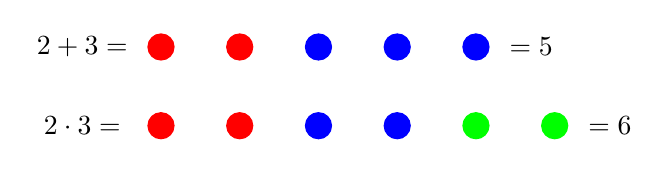
\begin{tikzpicture}
\node at (0,0) {$2+3 = $};
\node[draw, circle, fill, red] at (1,0) {};
\node[draw, circle, fill, red] at (2,0) {};
\node[draw, circle, fill, blue] at (3,0) {};
\node[draw, circle, fill, blue] at (4,0) {};
\node[draw, circle, fill, blue] at (5,0) {};
\node at (5.7,0) {$=5$};
\node at (0,-1) {$2\cdot 3 = $};
\node[draw, circle, fill, red] at (1,-1) {};
\node[draw, circle, fill, red] at (2,-1) {};
\node[draw, circle, fill, blue] at (3,-1) {};
\node[draw, circle, fill, blue] at (4,-1) {};
\node[draw, circle, fill, green] at (5,-1) {};
\node[draw, circle, fill, green] at (6,-1) {};
\node at (6.7,-1) {$=6$};
\end{tikzpicture}
\end{figure}

+ is associative immediately from the definitions. However, if $\omega$ is the order type of $\N$, then $1+\omega = \omega$ under the isomorphism ``subtract 1", however $\omega+1$ would have $\omega$ as an initial segment, and so $1+\omega \neq \omega+1$. As an exercise (see sheet 2), think about whether multiplication is associative, commutative, or distributive.

\subsection{Ordinal Arithmetic II - Attack of the Ordinals}
There is an alternative approach, using ideas of induction and recursion. First, we will need some preliminary ideas.

\begin{proposition}
\item
\begin{enumerate}
\item Let $\alpha$ be an ordinal. Then there is a least ordinal $\beta > \alpha$.
\item Let $X$ be a set of ordinals. then there is a least ordinal $\gamma$ with $\gamma >\delta$ or all $\delta \in X$.
\end{enumerate}
\end{proposition}
\begin{proof}
\item
\begin{enumerate}
\item Take $\beta$ to be $\alpha$ with a single additional element added greater than everything in $\alpha$.
\item Let $Y = \{I_{\delta} : \delta \in X\}$. Then $X$ is the set of order types of elements of $Y$ and the elements of $Y$ are nested sets of ordinals. So take $gamma$ to be the order type of $\bigcup_{\delta \in X} I_{\delta}$.
\end{enumerate}
\end{proof}

In \textit{1.}, we write $\beta = \alpha^{+}$, the \emph{successor} of $\alpha$. In \textit{2}, we write $\gamma = \sup(X)$, the \emph{supremum} of $X$. If $\alpha = \beta^{+}$ for some ordinal $\beta$, we say $\alpha$ is a \emph{successor ordinal}, and otherwise $\alpha$ is a \emph{limit ordinal}. For example, $0$ is a limit, $n \in \N$ is a successor, $\omega$ is a limit. Note that $\alpha$ is a limit if and only if $\alpha = \sup(I_{\alpha})$.

When doing induction or recursion for ordinals, we often deal with successors and limits in separate cases. We often treat $0$ as different to other limits as well.

We can then define addition and multiplication for ordinals recursively as follows:
\begin{itemize}
\item $\alpha + 0 = \alpha$
\item $\alpha + \beta^{+} = (\alpha + \beta)^{+}$
\item $\alpha + \gamma = \sup\{\alpha + \delta : \delta < \gamma\}$
\item $\alpha \cdot 0 = 0$
\item $\alpha \cdot \beta^{+} = \alpha \cdot \beta + \alpha$
\item $\alpha \cdot \gamma = \sup\{\alpha\delta : \delta < \gamma\}$.
\end{itemize}

However we have a problem - recursion doesn't work here since the ordinals do not form a set. We can get around this though.

Let $\alpha$ be an ordinal and suppose we want to define $\alpha + \beta$ for all ordinals $\beta$. Given an ordinal $\gamma$ we can define $\alpha + \beta$ recursively for all $\beta \in I_{\gamma}$ as above, since $I_{\gamma}$ is a set. Suppose we restrict this definition to $\beta \in I_{\gamma'}$ for some $\gamma' < \gamma$. Then this is the same as the direct definition on $I_{\gamma'}$. Hence we have uniquely defined $\alpha + \beta$ for all $\beta$, since $\beta \in I_{\beta^+}$.

What about induction? Suppose we have some statement $p(\alpha)$ about an ordinal $\alpha$ such that for all $\alpha$, $(\forall \beta  \alpha, p(\beta)) \implies p(\alpha)$. Take an ordinal $\alpha$. By induction, for all $\gamma \in I_{\alpha^+}, p(\gamma)$. Hence $p(\alpha)$. So in fact $p(\alpha)$ holds for all ordinals $\alpha$.

\begin{lemma}
Let $\alpha, \beta, \gamma$ be ordinals. Then
\begin{enumerate}
\item $\beta \leq \gamma \implies \alpha + \beta \leq \alpha+\gamma$
\item $\beta < \gamma \implies \alpha + \beta < \alpha + \gamma$
\item $\gamma$ a non zero limit ordinal $\implies \alpha+\gamma$ a limit ordinal
\end{enumerate}
\end{lemma}
\begin{proof}
\item
\begin{enumerate}
\item We do this by induction on $\gamma$. If $\beta = \gamma$ then it is obvious, so assume $\beta < \gamma$. For $\gamma = 0$, there is no such $\beta$, so done. Otherwise, if $\gamma=  \delta^+, \beta < \delta^+ \implies \beta \leq \delta \implies \alpha + \beta \leq \alpha + \delta < (\alpha + \delta)^+ = \alpha + \delta^+ = \alpha+\gamma$. The final case is $\gamma$ is a non-zero limit. Then $\beta < \gamma \implies \alpha+\gamma = \sup\{\alpha + \delta : \delta < \gamma\} \geq \alpha+\beta$.

\item Suppose $\beta < \gamma$. Then $\beta^+ \leq \gamma$, so $\alpha + \beta < (\alpha + \beta)^+ = \alpha +\beta^+ \leq \alpha +\gamma$.

\item Suppose instead that $\alpha + \gamma = \delta^+$ for some $\delta$. Then $\delta < \alpha + \gamma = \sup\{\alpha + \epsilon : \epsilon < \gamma\}$, so $\delta < \alpha + \epsilon$ for some $\epsilon < \gamma$. As $\gamma$ is a limit, then $\epsilon^{+} < \gamma$. Then $\alpha + \gamma = \delta^+ \leq (\alpha + \epsilon)^+ = \alpha + \epsilon^+ < \alpha + \gamma$ by \textit{2.}. \contr
\end{enumerate}
\end{proof}
\begin{proposition}
Let $\alpha, \beta, \gamma$ be ordinals. Then $(\alpha+\beta)+\gamma = \alpha + (\beta + \gamma)$
\end{proposition}
\begin{proof}
We use induction on $\gamma$. In the case $\gamma = 0, (\alpha + \beta) + 0 = \alpha + \beta = \alpha + (\beta + 0)$.

If $\gamma = \delta^+$, then $(\alpha + \beta) + \delta^+ = ((\alpha+\beta) + \delta)^+ = (\alpha + (\beta + \delta))^+ = \alpha + (\beta+\delta)^+ = \alpha + (\beta+ \delta^+)$.


If $\gamma$ is a non-zero limit, then $(\alpha + \beta) + \gamma = \sup(X)$ where $X = \{(\alpha+\beta)+\delta : \delta < \gamma\} = \{\alpha + (\beta+\delta) : \delta < \gamma\}$. Meanwhile, by \textbf{2.10} part 3, $\beta + \gamma$ is a limit, and so $\alpha + (\beta+ \gamma) = \sup(Y)$ where $Y = \{\alpha + \epsilon : \epsilon < \beta + \gamma\}$. If $\delta < \gamma$ then by \textbf{2.10} part 2, $\beta+ \delta < \beta + \gamma$ so $X \subset Y$, and so $(\alpha + \beta) + \gamma \leq \alpha + (\beta+\gamma$. On the other hand, if $\zeta \in Y$, then $\zeta = \alpha + \epsilon$ for some $\epsilon < \beta + \gamma = \sup\{\beta + \delta : \delta  < \gamma\}$. Hence $\epsilon \leq \beta + \delta$ for some $\delta < \gamma$. Let $\eta = \alpha + (\beta + \delta)$. Then \textbf{2.10} part 1, $\eta \geq \zeta$ and also $\eta \in X$. Hence $\sup(X) \geq \sup(Y)$, so $(\alpha + \beta) + \gamma \geq \alpha + (\beta+\gamma)$, and so $(\alpha+\beta)+\gamma = \alpha +(\beta+\gamma)$.
\end{proof}

The definition in this section is the \emph{inductive} definition of arithmetic, whilst the one in the previous section was the \emph{synthetic} definition. It is often better to work with the synthetic definition than the inductive one. Fortunately however, they coincide.

\begin{proposition}
The synthetic and inductive definitions of ordinal addition coincide.
\end{proposition}
\begin{proof}
Let $+$ denote the synthetic definition. Then for all $\alpha$, $\alpha + 0 = \alpha$, and also $\alpha+\beta^+ = \leftarrow \alpha \rightarrow \leftarrow \beta \rightarrow \cdot = (\alpha+\beta)^+$

Finally, if $\alpha$ is an ordinal and $\gamma$ is a non-zero limit ordinal, then $\alpha + \gamma = \leftarrow \alpha \rightarrow \leftarrow \sup\{\delta:\delta<\gamma\}\rightarrow = \sup(\alpha+\delta: \delta <\gamma\}$, by noting that $\delta$ is the order type of $I_{\delta}$, and the $I_{\delta}$ are nested so $\sup \leftrightarrow \cup$.

Hence by induction on $\beta$ the definitions agree on $\alpha + \beta$.
\end{proof}
\begin{proposition}
The synthetic and inductive definitions of ordinal multiplication coincide.
\end{proposition}
\begin{proof}
Left as an exercise for sheet 2.
\end{proof}

Can we define ordinal exponentiation? It's clear what to do inductively, but not so much synthetically. We define:
\begin{itemize}
\item $\alpha^0 = 0^+$
\item $\alpha^{\delta^+} = \alpha^{\delta}\alpha$
\item $\alpha^{\beta}$ for $\beta$ a non-zero limit to be $\sup\{\alpha^\delta: \delta<\beta\}$.
\end{itemize}

\subsection{Uncountable Ordinals}
In \textbf{\textsection 1.4} our list of indices $0,1,2,\ldots, \omega,\ldots, \omega 2, \ldots, \epsilon_0$ are some ordinals. We've found lots of them, but in fact only countably many - $\epsilon_0 = \sup\{\omega, \omega^{\omega},\ldots\}$. Since $\alpha$ is the order type of $I_{\alpha}$, equivalently each of these ordinals is countable. However, there are more:
\begin{proposition}
There exists an uncountable ordinal.
\end{proposition}
\begin{proof}
Let $X \subset \powset(\N \times \N)$ be the set of all well-orderings of subsets of $\N$. Let $Y = \{\ord(x)  : x \in X\}$. Then $Y$ is precisely the set o countable ordinals. Let $\omega_1 = \sup(Y)$. Suppose $\omega_1$ is countable. Then $\omega_1 \in Y$ and the proper initial segment $Y_{(<\omega_1)}$ has the same order type as $Y$. \contr
\end{proof}
A couple of remarks:
\begin{itemize}
\item $\omega_1$ is the least uncountable ordinal.
\item The ordinal $\omega_1$ is not the supremum of any countably set of countable ordinals. Indeed, if $Z$ is a countable set of countable ordinals, then $\sup Z$ is the order-type of $\bigcup_{\alpha \in Z}I_{\alpha}$, a countable union of countable sets.
\end{itemize}
\begin{theorem}
Let $S$ be a set. Then there exists an ordinal $\gamma$ with no injection $\gamma \to S$.
\end{theorem}
\begin{proof}
Same as the previous proposition with $\N$ replaced by $S$.
\end{proof}
Theorem \textbf{2.15} is called \emph{Hartog's Lemma}. This makes sense of the statement in \textbf{\textsection 1.4} that we eventually run out of stuff, with a formal proof to follow in the next section.

\section{Posets and Zorn's Lemma}
A \emph{\underline{p}artially \underline{o}rdered \underline{set} (poset)} is a set $P$ with a relation $\leq$ satisfying:
\begin{enumerate}
\item $(x\leq y, y\leq z) \implies x \leq z$
\item $\forall x \in P, x\leq x$
\item $(x\leq y, y\leq x) \implies y = x$
\end{enumerate}
If $(P, \leq)$ is a poset and we define $x<y$ to mean $x \leq y$ and $x \neq y$, then
\begin{enumerate}
\item $(x<y, y<z) \implies x < z$
\item $x \nless x$
\end{enumerate}

Conversely, we can check that if $P$ is a set and $<$ is a relation on $P$ satisfying the above then $\leq$ gives a partial order on $P$. We use $>, \geq$ in the obvious way.

A \emph{Hasse diagram} of $(P, \leq)$ consists of a point for each $x \in P$ and line upwards from $x$ to $y$ if $y$ \emph{covers} $x$, i.e. that $y > x$ and there is no $z$ with $y > z > x$.

\hspace*{-1em}\underline{Examples}
\begin{enumerate}
\item Any totally ordered set is a poset.
\item Any subset of a poset is a poset.
\item For any set $X$, $\powset(X)$ is a poset under inclusion.
\item In a similar vein, take $\N$ with $|$ (divides). This is a poset.
\item We have the finite set with Hasse diagram given by:
\begin{center}
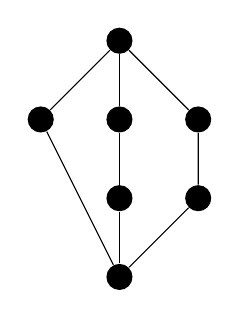
\begin{tikzpicture}
\node[circle, fill] (a) at (0,3) {};
\node[circle, fill] (b) at (-1,2) {};
\node[circle, fill] (c) at (0,2) {};
\node[circle, fill] (d) at (1,2) {};
\node[circle, fill] (e) at (0,1) {};
\node[circle, fill] (f) at (1,1) {};
\node[circle, fill] (g) at (0,0) {};
\draw (a) -- (b) -- (g);
\draw (a) -- (c) -- (e) -- (g);
\draw (a) -- (d) -- (f) -- (g);
\end{tikzpicture}
\end{center}
\end{enumerate}

Let $(P, \leq)$ be a poset. We say that $x \in P$ is \emph{greatest} if for all $y \in P, y \leq x$. We say that $x \in P$ is \emph{maximal} if for all $y \in P$, $y \geq x \implies y = x$. If $S \subset P$, an \emph{upper bound} for $S$ is an $x \in P$ such that $y \in S \implies y \leq x$. We can similarly define \emph{least}, \emph{minimal}, and \emph{lower bound}. If $S$ has a least upper bound we denote it by $\sup(S)$ or by $\bigvee S$, read ``join $S$". Similarly, if we have a greatest lower bound or infimum of $S \subseteq P$, we denote it by $\inf(S)$ or $\bigwedge S$, read ``meet $S$". We have the diagram:
\begin{center}
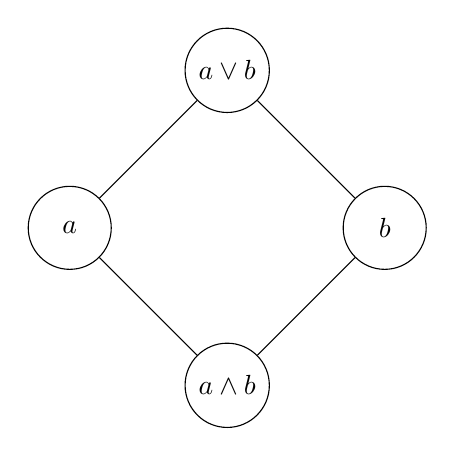
\begin{tikzpicture}
\node[circle, draw, minimum size=3em] (v) at (0,2) {$a \vee b$};
\node[circle, draw, minimum size=3em] (a) at (-2,0) {$a$};
\node[circle, draw, minimum size=3em] (b) at (2,0) {$b$};
\node[circle, draw, minimum size=3em] (n) at (0,-2) {$a \wedge b$};
\draw (v) -- (a) -- (n) (v) -- (b) -- (n);
\end{tikzpicture}
\end{center}
\hspace*{-1em}\underline{Examples:}
\begin{enumerate}
\item In $(\powset S, \subseteq)$, $S$ is greatest and $\emptyset$ is least.
\item In $(\N, \leq)$, $0$ is least. There is no greatest or maximal element.
\item Take the finite set with diagram given by:\\
\begin{minipage}{0.2\textwidth}
\centering
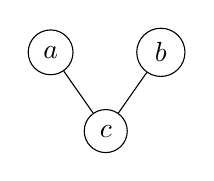
\begin{tikzpicture}
\node[circle, draw] (a) at (-0.7,1) {$a$};
\node[circle, draw] (b) at (0.7,1) {$b$};
\node[circle, draw] (c) at (0,0) {$c$};
\draw (a) -- (c) (b) -- (c);
\end{tikzpicture}
\end{minipage}
\begin{minipage}{0.5\textwidth}
We have $a$ is maximal, but $a$ is not greatest since $a \ngeq b$. $b$ is maximal as well. $c$ is both minimal and least.
\end{minipage}
\end{enumerate}
Note that $a$ greatest implies that $a$ is maximal, and if $P$ has a greatest element then it must be unique. If every subset of $P$ has a supremum then we say that $P$ is \emph{complete}. If $P$ is complete then $P$ is non-empty, as $\bigvee\emptyset \in P$. In fact, $\bigvee\emptyset$ is the least element of $P$. $P$ also has a greatest element, $\bigvee P$.

\hspace*{-1em}\underline{Examples:}
\begin{enumerate}
\item $(\powset S, \subseteq)$ is complete. $\bigvee \mathcal{A} = \bigcup_{A \in \mathcal{A}} A, \bigwedge \mathcal{A} = \bigcap_{A \in \mathcal{A}} A$.
\item $([0,1], \leq)$ is complete.
\item $(\R, \leq)$ is not complete.
\end{enumerate}
If $(P, \subseteq)$ is a poset then a \emph{chain} is a subset $C \subseteq P$ such that for all $x, y \in C$ either $x \leq y$ or $y \leq x$. If every chain has a supremum, we say that $P$ is \emph{chain-complete.} Note again that chain complete implies nonempty since the empty set is a chain.

\hspace*{-1em}\underline{Examples:}
\begin{enumerate}
\item In $(\N,1)$, the set $\{4^n : n \in \N\}$ is a chain.
\item In $(\R, \leq)$, $\Q$ is a chain, and so is $\R$.
\end{enumerate}

A \emph{lattice} $L$ is a poset in which every finite subset has both a supremum and an infimum. For $a, b \in L$, we write $a \vee b = \bigvee \{a, b\}$ and $a \wedge b = \bigwedge \{a, b\}$. Note that $L$ has a least element $\bigwedge \emptyset$ and a greatest element $\bigvee \emptyset$. We say that a lattice $L$ is a \emph{Boolean algebra} if:
\begin{enumerate}
\item For all $a,b,c \in L$, $a \wedge (b \vee c) = (a \wedge b)\vee(a \wedge c)$
\item For all $a,b,c \in L$, $a \vee (b \wedge c) = (a \vee b) \wedge (a \vee c)$
\item For all $a \in L$ there is $b \in L$, $a \vee b = \bigwedge \emptyset, a \wedge b = \bigvee \emptyset$
\end{enumerate}
These rules are essentially saying $L$ behaves like a powerset, with $\wedge$ corresponding to $\cap$ and $\vee$ corresponding to $\cup$. Then the first two rules are de Morgan's laws, and the third is the notion of a complement.

\subsection{Zorn's Lemma}
\begin{figure}[H]
\centering
\begin{tikzpicture}[scale=5]
\tikzset{rotate=-45}
\fill [MaterialYellow500] (0, 0) ellipse [x radius=1/3, y radius=  1];
\fill [MaterialYellow500] (0, 0) ellipse [x radius=3/4, y radius=7/8];
\fill [MaterialYellow600] (270:1/3 and   1) arc (270:450:1/3 and   1);
\fill [MaterialYellow600] (270:3/4 and 7/8) arc (270:450:3/4 and 7/8);
\begin{scope}[shift=(90:9/10), rotate=-135]
\fill [MaterialGreen500] 
  (0,0) arc (45:135:1/2 and 4/5) arc (225:315:1/2 and 3/5);
\fill [MaterialGreen700] 
  (0,0) arc (45:135:1/2 and 4/5) -- cycle;
\tikzset{rotate=90, scale=3/4}
\fill [MaterialGreen500] 
  (0,0) arc (45:135:1/2 and 4/5) arc (225:315:1/2 and 3/5);
\fill [MaterialGreen700] 
  (0,0) arc (45:135:1/2 and 4/5) -- cycle;
\end{scope};
\end{tikzpicture}
\caption{Zorn's Lemon}
\end{figure}
\begin{theorem}[Zorn's Lemma]
Let $(P, \leq)$ be a poset in which every chain has an upper bound. Then $P$ has a maximal element.
\end{theorem}
The idea is that, if not, we can take $x_0$ to be the upper bound of the empty set, then if $x_0$ is not maximal there is $x_1 > x_0$, and then we get another chain indexed by the ordinals, and eventually run out of stuff.
\begin{proof}
Suppose $P$ has no maximal element. Then for any $x \in P$, we can find $x' \in P$ with $x' > x$. Moreover, for any chain $C \subseteq P$ we can find $C^{\ast} \in P$ such that for all $x \in C$, $C^{\ast} > x$, for instance take $y$ to be an upper bound for $C$ and let $C^{\ast} = y'$.

By Hartog's Lemma, we can find an ordinal $\gamma$ such that there is no injection from $\gamma \to P$.

Recursively for $\alpha < \gamma$ define $x_{\alpha}$ as follows:
\begin{itemize}
\item[$\alpha=0$:] $x_0 = \emptyset^{\ast}$ - we can use any element of $P$
\item[$\alpha=\beta^+:$] $x_{\beta^+} = x_{\beta}'$
\item[Otherwise:] $\alpha$ is a non-zero limit, so let $x_{\alpha} = \{x_{\delta} : \delta < \alpha\}^{\ast}$.
\end{itemize}
We can do this because $\{x_\delta : \delta < \alpha\}$ is a chain as $x_{\zeta} > x_{\xi} \iff \zeta > \xi$, and the ordinals are totally ordered.

Then $\alpha \mapsto x_{\alpha}$ is an injection $I_\gamma \to P$, and $I_\gamma \cong \gamma$. \contr
\end{proof}
But can we actually let $x_{\alpha} = \{x_{\delta} : \delta < \alpha\}^{\ast}$? Even though we know the thing on the right is a chain, we don't know that until we're halfway through the recursion - when we define what $x_\alpha$ will be, we are saying its the star of something that may or may not be a chain. It is only once we find out what this something is that we know it is indeed a chain and we can take a star of it, and this first assignment is slightly dodgy. To get around this, we use the technical fix of cabbages:

\textbf{Cabbages.} Take something not in $P$, for instance a cabbage that we happen to have lying around. For $\alpha < \gamma$, define $x_\alpha \in P\cup \{$cabbage$\}$ exactly as above, except for $\alpha$ a non-zero limit.

Then set for $\alpha$ a non-zero limit, let $x_\alpha = \begin{cases} \{x_\delta:\delta<\alpha\}^{\ast} & \text{this set is a chain}\\ \text{cabbage} & \ow\end{cases}$, and also define cabbage$' = $ cabbage. By induction, we don't get any cabbage. In these proofs, cabbages are implicitly assumed.

\subsection{Applications of Zorn's Lemma}
The general method of applying Zorn's Lemma is as follows:
\begin{enumerate}
\item Define a suitable poset.
\item Check every chain has an upper bound.
\item Use Zorn to find a maximal element $x$.
\item Check $x$ is the thing we are looking for.
\end{enumerate}
It is not unusual for most of the work to come in step 4.
\begin{corollary}
Let $P$ be a set of primitive propositions, and let $S \subset L = L(P)$ be consistent. Then there is a consistent $\bar{S} \subset L$ with $S \subset \bar{S}$ and for all $p \in L$, $p \in \bar{S}$ or $\neg p \in \bar{S}$.
\end{corollary}
\begin{proof}
Let $X$ be the poset  $\{R\subset L | R$ consistent and $S \subset R\}$, ordered by $\subset$. Let $\mathscr{C} \subset X$ be a chain. If $\mathscr{C} = \emptyset$ then $S \in X$ is an upper bound for $\mathscr{C}$. 

Suppose $\mathscr{C} \neq \emptyset$. Let $Q = \bigcup_{R \in \mathscr{C}} R$. Then for all $R \in \mathscr{C}, R \subset Q$. As $\mathscr{C} \neq \emptyset$, there exists $R \in \mathscr{C}$ and $S \subset R \subset Q$. Suppose that $Q$ is inconsistent, i.e. that $Q \vdash \bot$. As proofs are finite, there are some $q_1, \ldots, q_n \in Q$ such that $\{q_1, \ldots, q_n\}\vdash\bot$. For each $i$, pick $R_i \in \mathscr{C}$ with $q_i \in R_i$. As $\mathscr{C}$ is a chain and there are only finitely many of $R_1, \ldots, R_n$, there exists $j$ such that $R_i \subseteq R_j$ for all $i$. Then $q_1, \ldots, q_n \in R_j$, and so $R_j \vdash \bot$. \contr

Hence $Q$ is consistent. Thus $Q \in X$ is an upper bound for $\mathscr{C}$. By Zorn's lemma, $X$ has a maximal element $\bar{S}$. Let $p \in L$ and suppose $p \notin \bar{S}$. Then $\bar{S} \cup \{p\}$ is inconsistent, as otherwise $\bar{S} \cup \{p\} \in X$ with $\bar{S} \subsetneq \bar{S}\cup\{p\}$. That is, $\bar{S}\cup\{p\} \vdash \bot$, and so by the deduction theorem $\bar{S} \vdash (p \implies \bot)$, i.e. $\bar{S} \vdash \neg p$. So, similarly to the above, $\neq p \in \bar{S}$.
\end{proof}
This fills the gap in the proof of the Model Existence Lemma, thus finishing the proof of the completeness theorem. It is very common when using Zorn to consider a poset of the form $(X, \subseteq)$ where $X \subseteq \powset(A)$ for some set $A$. If $\mathscr{C}$ is a chain in $X$, an obvious guess for an upper bound for $\mathscr{C}$ is $Q = \bigcup_{R \in \mathscr{C}} R$. Clearly for all $R \in \mathscr{C}$, $R \subseteq Q$, but often work is needed to show that $Q \in X$, so that $Q$ is genuinely an upper bound for $\mathscr{C}$ in $X$. Also, care must be taken to remember that $\emptyset$ si a chain, and often needs t be considered separately.

\begin{corollary}
Every vector space has a basis.
\end{corollary}
\begin{proof}
Let $V$ be a vector space over a field $k$. Let $P = \{S \subseteq V | S$ is linearly independent$\}$, ordered by $\subseteq$. Let $\mathscr{C} \subseteq P$ be a chain, and let $R = \bigcup_{S \in \mathscr{C}}S$. Suppose that $R$ is linearly dependent. Then there are some $n \in \N\setminus\{0\}$, and some distinct $v_1, \ldots, v_n \in R$ and some $\lambda_1, \ldots, \lambda_n \in k$ with $\sum_{i=1}^n \lambda_i v_i = 0$. For each $i$, pick $S_i \in \mathscr{C}$ with $v_i \in S_i$. As $\mathscr{C}$ is a chain, there is some $j$ for which $S_i \subseteq S_j$ for all $i =1, \ldots, n$. Then $v_1, \ldots, v_n \in S_j$ , so $S_j$ is linearly dependent. \contr

Hence $R$ is linearly independent, and so $R$ is an upper bound for $\mathscr{C}$. By Zorn, $P$  has a maximal element $B$. Certainly $B$ is linearly independent. Suppose there is some $v \in V \setminus \spann{B}$. We show that $B \cup\{v\}$ is linearly independent. Indeed, if not then we have a linear combination $\mu v - \sum_{i=1}^n \lambda_i b_i = 0$, where $b_i \in B$, but then $v = \sum \mu^{-1}\lambda_i b_i \in \spann{B}$\contr. But then $B\cup\{v\} \in P$, and $B \subsetneq B\cup\{v\}$, \contr maximality of $B$.

So $B$ is a linearly independent set spanning $V$, and so $B$ is a basis for $V$.
\end{proof}

\begin{corollary}[Bourbaki-Witt Theorem]
Let $(X, \leq)$ be a poset, and let $X$ be chain-complete, and $f: X \to X$ be such that for all $x \in X, f(x) \geq x$. Then $f$ has a fixed point.
\end{corollary}
\begin{proof}
By Zorn $X$ has a maximal element $x$. Then $f(x) \in X, f(x) \geq x$, so by maximality $f(x) = x$.
\end{proof}

\begin{corollary}[Well-Ordering Principle]
Every set can be well-ordered.
\end{corollary}
\begin{proof}
Let $X$ be a set. Let $P = \{(Y,R) | Y\subset X$ and $R$ is a well-ordering of $Y\}$. Define $(Y,R)\leq (Z,S)$ if $Y \subset Z$ and $R,S$ agree on $Y$, and $Y$ is an initial segment of $Z$ in $S$. Then $(P, \leq)$ is a poset. Let $\mathscr{C} \subset P$ be a chain, say $\mathscr{C} = \{(Y_i, R_i) | i \in I\}$. Let $Y = \bigcup_{I \in I} Y_i$. Define a relation $R$ on $Y$ as follows: if $x,y \in Y$ then choose $j, k \in I$ such that $x \in Y_j$ and $y \in Y_k$. If $Y_j \subset Y_K$ then $xRy \iff xR_k y$, otherwise $Y_k \subset Y_j$ in which case $xRy \iff xR_j y$.

It is easy to show that $R$ is a total ordering of $Y$. We must show further that it is a well ordering. Let $A \subset Y$ with $A \neq \emptyset$. Then there exists $x \in A$, so $x \in Y_{\ell}$ for some $\ell \in I$, so $A \cap Y_{\ell} \neq \emptyset$. But we know $Y_{\ell}$ is well ordered by $R_{\ell}$, so $A \cap Y_{\ell}$ has an $R_\ell$-least element, $z$, say. So $z$ is also the $R$-least element of $A \cap Y_\ell$, and hence $R$ is a well ordering of $Y$.

Thus, $(Y,R) \in P$ and is an upper bound for $\mathscr{C}$. Then by Zorn, $P$ has a maximal element $(Z,S)$. Suppose there is some $x \in X \setminus Z$. Then $S \cup \{(z, x) | z \in Z \cup \{x\}\}$ is a well ordering of $Z \cup \{x\} \supsetneq Z$, and $Z$ is an initial segment. \contr

Hence $Z = X$ and $S$ is a well ordering of $X$.
\end{proof}
\subsection{The Axiom of Choice}
In the proof of Zorn's Lemma (ZL), we had to make infinitely many arbitrary choices, e.g. for all $x \in X$, pick some $x' > x$. We've done this quite a bit throughout tripos, for instance in IA Numbers and Sets, when we proved that a countable union of countable sets is countable by picking an ordering of each set so that we can move along the list diagonally.

\begin{axiom}[The Axiom of Choice]
Let $\{X_i | i \in I\}$ be a set of non-empty sets. Then there exists a function $f: I \to \bigcup_{i \in I}X_i$ such that, for all $i \in I$, $f(i) \in X_i$.
\end{axiom}
The function $f$ is sometimes called a \emph{choice function} for the collection $\{X_i|i \in I\}$.

The axiom of choice (AC) has a different feel from our other usual assumptions about sets, e.g. it doesn't explicitly construct anything, so it can be of interest to see if we've used it. For example we used AC when proving Zorn's Lemma, but it might be an interesting question to ask if we needed to. What does this even mean? To give a sensible answer, we'd need to axiomatise set theory, and think about proof systems, and then show that if we only assume axioms other than AC then Zorn's Lemma would no longer be a theorem. This would take a lot of work (c.f. Russell and Whitehead, Principia Mathematica). For now, we will do a similar thing - assume Zorn's Lemma and use it to prove AC.
\begin{proof}
Let $\{X_i | i \in I\}$ be a collection of non-empty sets, and let
\begin{align*}
P = \left\{\left.g \subset \powset\left(I \times \bigcup_{i \in I} X_i \right) \right| g:J\to \bigcup_{i\in I}X_i, J \subseteq I; \forall i \in \dom(g), g(i) \in X_i\right\}
\end{align*}
ordered by inclusion. Not $g \subset g'$ means $\dom g \subset \dom g'$ and $g'|_{\dom g} = g$. Let $\mathscr{C}$ be a chain in $P$. Let $h = \bigcup_{g \in \mathscr{C}} g$. Then $h$ is a function with $\dom h = \bigcup_{g\in \mathscr{C}} \dom g$.

Moreover, $h \in P$ and is an upper bound for $\mathscr{C}$. So by Zorn $P$ has a maximal element $f$. Suppose $i \in I \setminus \dom f$. Pick $x \in X_i$\footnote{We can do this without using AC since we are only making one choice, and that is precisely what it means for a set to be nonempty - we can pick an element from it}. Then $f \subsetneq f \cup \{(i, x)\} \in P$. \contr
So $f$ is our required choice function.
\end{proof}

However, in the case where the index set $I$ is finite, AC \textit{does} follow from our assumptions. For instance, if $I = \{a,b,c\}$, then if we have nonempty sets $X_a, X_b, X_c$, we can, by definition write $x_a \in X_a, x_b \in X_b, x_c \in X_c$. Then we can write down our choice function $ = \{(a, x_a), (b, x_b), (c, x_c)\}$.

Another way of thinking of the axiom of choice is that, if $X_i \neq \emptyset$ for all $i \in I$, then the Cartesian product $\prod_{i \in I} X_i \neq \emptyset$.

Do we need AC to prove the well ordering principle? Note that we can prove the axiom of choice from the well ordering principle by well ordering $\bigcup_i X_i$ and choosing the least element of $X_i$.

Bourbaki-Witt does not need the axiom of choice though.

\section{Cardinals}
Let $X$ and $Y$ be sets. If there is a bijection $X \to Y$ we say $X,Y$ \emph{have the same cardinality}, and write $|X| = |Y|$.

Note that $|X|=|X|; |X|=|Y|\implies|Y|=|X|$, and $(|X|=|Y|,|Y|=|Z|) \implies |X|=|Z|$.

We want to define cardinals in such a way that every set $X$ has the same cardinality as precisely one cardinal. By WOP every set $X$ can be well-ordered, so $X$ has the same cardinality as some ordinal.

We then define the \emph{cardinality} $\card(X)$ to be the least ordinal with the same cardinality as $X$. 

If $X, Y$ are sets, then we write $|X|\leq |Y|$ to mean there is an injection from $X$ to $Y$. Clearly $|X|\leq |X|$, and $(|X|\leq |Y|, |Y|\leq |Z|) \implies |X|\leq|Z|$. Moreover, by Cantor-Schr\"oder-Bernstein, if $|X|\leq |Y|$ and $|Y| \leq |X|$, then $|X|=|Y|$.

But then the question is what are the cardinals? We define an ordinal $\alpha$ to be \emph{initial} if for all $\beta > \alpha$ there is no bijection $\beta \to \alpha$. For example, 0,1,2,3,\ldots are all initial ordinals. $\omega, \omega_1$ are also initial ordinals. However, no ordinal $\alpha$ with $\omega <\alpha <\omega_1$ is initial.

For $\alpha$ an ordinal, we can define $\omega_\alpha$ recursively:
\begin{itemize}
\item[$\alpha=0$:] $\omega_0 = \omega$
\item[$\alpha=\beta^+$:] $\omega_{\beta^+}$ is the least ordinal with no injection to $\omega_{\beta}$ which exists by Hartog's lemma.
\item[$\alpha$ limit:] $\omega_\alpha = \sup\{\omega_{\delta} : \delta < \alpha\}$.
\end{itemize}
For every $\alpha$, $\omega_\alpha$ is an infinite initial ordinal. We can also prove the converse: it is easy to show by induction that, for all $\alpha, \omega_\alpha \geq \alpha$.

Now let $\alpha$ be an infinite initial ordinal. Then it is easy to check that, if $\delta$ is least with $\omega_\delta \geq \alpha$, then $\alpha = \omega_\delta$.

We then write $\aleph_\alpha = \card(\omega_\alpha)$, so that the cardinals are $0,1,2,\ldots$ and the infinite cardinals, the $\aleph_\alpha$ for $\alpha$ ordinals. We have two different notations for the same thing because sometimes we want to think about it as a cardinal and sometimes as an ordinal. The important thing about cardinals is that there is precisely one of each cardinality - the fact that we've defined them as ordinals to make this work is not important.

\subsection{Cardinal Arithmetic}
Let $\kappa, \lambda$ be cardinals. We define:
\begin{itemize}
\item $\kappa + \lambda = \card(\{0\}\times \kappa \cup \{1\}\times \lambda\}$
\item $\kappa\lambda = \card(\kappa\times \lambda)$
\item $\kappa^{\lambda} = \card(\{f| f:\lambda\to\kappa\})$
\end{itemize}
Warning: this is not the same definition of exponentiation as for ordinals, as for instance $2^{\omega_0} = \omega_0$, but $2^{\aleph_0} = \card(\powset(\N)) \neq \card(\N) = \aleph_0$.

\begin{proposition}
\item
\begin{enumerate}
\item $(\kappa + \lambda) + \mu = \kappa + (\lambda + \mu)$
\item $\kappa + \lambda = \lambda + \kappa$
\item $(\kappa\lambda)\mu = \kappa(\lambda\mu)$
\item $\kappa\lambda = \lambda\kappa$
\item $\kappa(\lambda+\mu) = \kappa\lambda + \kappa\mu$
\item $(\kappa\lambda)^\mu = \kappa^\mu\lambda^\mu$
\item $\kappa^{\lambda + \mu} = \kappa^{\lambda}\kappa^\mu$
\item $(\kappa^\lambda)^\mu = \kappa^{\lambda\mu}$.
\end{enumerate}
\end{proposition}
This is left as an exercise, but we'll illustrate an example here. For, say, \textit{5.}, we need to find a bijection:
\begin{align*}
f:\kappa\times\left((\{0\}\times\lambda)\cup(\{1\}\times \mu)\right) \to \left(\{0\}\times(\kappa\times\lambda)\right)\cup\left(\{1\}\times(\kappa\times\mu)\right)
\end{align*}
So take $f(x,(n,y)) = (n,(x,y))$ - this does the job.

In fact, addition and multiplication are easy because:
\begin{proposition}
Let $\kappa$ be an infinite cardinal. Then $\kappa\kappa =\kappa$.
\end{proposition}
\begin{proof}
We have $\kappa = \aleph_\alpha$ for some ordinal $\alpha$. Think of $\kappa$ as the initial ordinal $\omega_\alpha$, so it is well-ordered.

We then need to show that $\card(\omega_\alpha \times \omega_\alpha) = \card(\omega_\alpha)$.

Well order $\omega_\alpha \times \omega_\alpha$ by $(x,y) < (z,w)$ if:
\begin{itemize}
\item $\max(x,y) < \max(z,w)$, or
\item $y = w \geq x,z$ and $ x < z$, or
\item $x = z > y,w$ and $y < w$, or
\item $y = z, y \geq x, z > w$.
\end{itemize}
This looks like a mess, but we can think of it more clearly with a picture:
\begin{figure}[H]
\centering
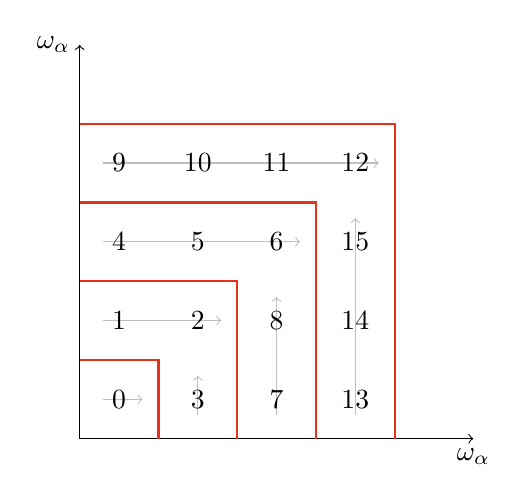
\begin{tikzpicture}
\draw[->] (0,0) -- (5,0) node[below] {$\omega_\alpha$};
\draw[->] (0,0) -- (0,5) node[left] {$\omega_\alpha$};
\draw[lightgray,->] (0.3,0.5)--(0.8,0.5);
\draw[lightgray,->] (0.3,1.5)--(1.8,1.5);
\draw[lightgray,->] (1.5,0.3)--(1.5,0.8);
\draw[lightgray,->] (0.3,2.5)--(2.8,2.5);
\draw[lightgray,->] (2.5,0.3)--(2.5,1.8);
\draw[lightgray,->] (0.3,3.5)--(3.8,3.5);
\draw[lightgray,->] (3.5,0.3)--(3.5,2.8);
\foreach \x [count = \i] in {0,1,4,9}{
	\node (\x) at (0.5,-0.5+\i) {\x};
}
\foreach \x [count = \i] in {3,2,5,10}{
	\node (\x) at (1.5,-0.5+\i) {\x};
}
\foreach \x [count = \i] in {7,8,6,11}{
	\node (\x) at (2.5,-0.5+\i) {\x};
}
\foreach \x [count = \i] in {13,14,15,12}{
	\node (\x) at (3.5,-0.5+\i) {\x};
} 
\draw[thick, red!60!brown] (1,0)--(1,1)--(0,1) (2,0)--(2,2)--(0,2) (3,0)--(3,3)--(0,3) (4,0)--(4,4)--(0,4);
\end{tikzpicture}
\end{figure}
In this well-ordering, what can we say about the order-type of $\omega_\alpha\times\omega_\alpha$?

Consider a proper initial segment $(\omega_\alpha \times \omega_\alpha)_{(<\delta)}$. As $\omega_\alpha$ is initial and hence a limit, $\delta = \beta \times \beta$ for some $\beta < \omega_\alpha$. Then, writing $I = (\omega_\alpha \times \omega_\alpha)_{(<\delta)}$, in fact $I \subset \beta \times \beta$. As $\omega_\alpha$ is initial, $\card(\beta) < \card(\omega_\alpha)$, so either $\beta$ is finite, in which case $\beta \times \beta$ is finite, or $\beta$ is infinite, in which case by the inductive hypothesis, $\card(\beta \times \beta) = \card(\beta)$.

In either case, $\card(\beta \times \beta) < \aleph_\alpha$, and so $\ord(I) < \omega_\alpha$. Hence $\card(\omega_\alpha\times\omega_\alpha) \leq \card(\omega_\alpha)$, so $\kappa\kappa \leq\kappa$. But clearly $\kappa \leq \kappa\kappa$, and so $\kappa\kappa = \kappa$ as claimed.
\end{proof}
\begin{corollary}
Let $\kappa, \lambda$ be infinite cardinals. Then:
\begin{align*}
\kappa+\lambda = \kappa\lambda = \max(\kappa,\lambda)
\end{align*}
\end{corollary}
\begin{proof}
\textsc{Wlog} $\kappa \geq \lambda$. Then:
\begin{align*}
\kappa \leq \kappa+\lambda \leq \kappa+\kappa = 2\kappa \leq \kappa\lambda\leq \kappa\kappa =\kappa
\end{align*}
\end{proof}
\hspace*{-1em}\underline{Examples:}
\begin{enumerate}
\item $\card{\R} = \card{\powset(\N)} = 2^{\aleph_0}$.
\item Let $X$ be the set of real sequences. What is $\card(X)$? Well, $\card(X) = \card(\R^\N) = (2^{\aleph_0})^{\aleph_0}=2^{\aleph_0\aleph_0}=2^{\aleph_0}$, i.e. there is a bijection from the set of the reals to the set of real sequences.
\end{enumerate}
What about exponentiation? This turns out to be \underline{\underline{HARD}}. What is $2^{\aleph_0}$? We know that $2^{\aleph_0} = \aleph_\alpha$ for some $\alpha \geq 1$. We could guess that $2^{\aleph_0} = \aleph_1$, but it is impossible to prove one way or the other, even using the axiom of choice as we have been. We cannot prove that $\R$ has an uncountable subset that doesn't biject with $\R$.

One thing that is true: for any $\kappa, 2^{\kappa} > \kappa$. This is left as an exercise - show there is no bijection $\powset(X) \to X$ for any $X$.

\subsection{A Slight Remark on the Axiom of Choice}
This whole section has been heavily dependent on AC. We even needed AC to define what the cardinals are! In fact, without AC, we can still define a nice definition of cardinals and define arithmetic, with the basic properties still holding. However, we can no longer prove:
\begin{itemize}
\item Every infinite cardinal is $\aleph_\alpha$ for some ordinal $\alpha$
\item \textbf{4.2} and \textbf{4.3} only work for the $\aleph$ cardinals, but not necessarily for the other cardinals that might exist.
\item For cardinals $\kappa, \lambda$ we have either $\kappa \leq \lambda$ or $\lambda \leq \kappa$.
\end{itemize}
We can still prove that $(\kappa\leq\lambda, \lambda\leq\kappa)\implies \kappa=\lambda$.

\section{First Order Predicate Logic}
Keep the following two examples in mind:
\begin{itemize}
\item \underline{The Theory Of Groups (GT):} A group is a set $G$ with multiplication $m$, inverse $i$, and identity $e$ satisfying certain axioms. We can think of $m,i, e$ as functions. $m:G^2 \to G, i: G \to G, e: G^0 \to G$.
\item \underline{The Theory Of Posets (PT):} A poset is a set $P$ with a relation $\leq$ satisfying certain axioms. We have $\leq \subset P^2$.
\end{itemize}

A \emph{first order signature} is an ordered triple $\Sigma = (\Omega, \Pi, \alpha)$ where $\Omega$ and $\Pi$ are disjoint sets of symbols with $w, ', (, ), =, \implies, \bot, \forall \notin \Omega \cup \Pi$ and $\alpha : \Omega \cup \Pi \to \N$. We call $\Omega$ the set of \emph{function symbols}, $\Pi$ the set of \emph{relation symbols}, and $\alpha$ the \emph{arity function}.

\hspace*{-1em}\underline{Examples:}
\begin{itemize}
\item[GT:] $\Omega = \{m,i,e\}, \Pi = \emptyset, \alpha(m) = 2, \alpha(i) = 1, \alpha(e) = 0$.
\item[PT:] $\Omega = \emptyset, \Pi = \{\leq\}, \alpha(\leq) = 2$.
\end{itemize}

We then define the \emph{first-order language} $L = L(\Sigma) = L(\Omega, \Pi, \alpha)$ by a sequence of inductive definitions.

The \emph{variables} are defined inductively by:
\begin{itemize}
\item $w$ is a variable.
\item $x$ is a variable, so $x'$ is a variable.
\end{itemize}
So the variables are $w, w', w'', w''', \ldots$. Informally, we often use $w_0, w_1, \ldots$, or $x, y, z, \ldots$.

The \emph{terms} are defined inductively by:
\begin{itemize}
\item Every variable is a term.
\item If $f \in \Omega, \alpha(f) = n, t_1, \ldots, t_n$ are terms, then $ft_1t_2\ldots t_n$ is a term.
\end{itemize}
Informally, we'll sometimes add brackets and commas, i.e. $f(t_1, \ldots, t_n)$.

\hspace*{-1em}\underline{Examples:}
\begin{itemize}
\item[GT:] Some terms are $mxmmyzu$ or $mxiy$ or $e$\footnote{These are more commonly recognised as $(x\cdot ((y\cdot z)\cdot u))$ or $(x\cdot y^{-1})$ or $e$}
\item[PT:] The only terms are the variables - we have no function symbols.
\end{itemize}

The \emph{atomic formulae} are defined inductively by:
\begin{itemize}
\item $\bot$ is an atomic formula.
\item If $s,t$ are terms then $s=t$ is an atomic formula.
\item If $\varphi \in \Pi$ and $\alpha(\varphi) = n$ and $t_1,\ldots, t_n$ are terms, then $\varphi t_1\ldots t_n$ is an atomic formula.
\end{itemize}
Again, we often insert brackets and commas.

The \emph{formulae} are defined inductively by:
\begin{itemize}
\item Every atomic formula is a formula.
\item If $p,q$ are formulae then $(p \implies q)$ is a formula.
\item If $x$ is a variable and $p$ is a formula then $(\forall x)p$ is a formula.
\end{itemize}

\hspace*{-1em}\underline{Examples:}
\begin{itemize}
\item[GT:] $\left((\forall x)(mxx = e)\implies (\forall x)(x=y)\right)$ or $(\forall x)(y=z)$ or $mxy = e$.
\end{itemize}
 
Suppose that $p$ is a formula and $x$ is a variable that appears in $p$. We say an occurrence of $x$ in $p$ is \emph{bound} if it is within a subformula of the form $(\forall x)q$; it is \emph{free} otherwise. A formula with no free variables is called a \emph{sentence}.

\hspace*{-1em}\underline{Examples:}
\begin{itemize}
\item[GT:] $(\forall x)(\forall y)(\forall z)(mmxyz = mxmyz)$ is a sentence.
\item[GT:] $(\forall x)(x=y)$ - $x$ is bound and $y$ is free.
\item[GT:] We can do stupid things like $((x=y)\implies (\forall x)(x=z))$. The first $x$ is free, the second is bound.
\end{itemize}

The \emph{first order language} $L(\Sigma)$ is the set of formulae. A \emph{theory} is a set $T$ of sentences.

For instance, the \emph{language of groups} is generated by $\Omega = \{m,i,e\}, \Pi = \emptyset, \alpha(m) = 2, \alpha(i) = 1, \alpha(e) = 0$. The \emph{theory of groups} is:
\begin{align*}
T = \big\{&(\forall x)(\forall y)(\forall z)(mxmyz = mmxyz), \tag{associativity}\\
&(\forall x)(mxe = x), \tag{identity}\\
&(\forall x)(mxix = e)\big\} \tag{inverses}
\end{align*}
We sometimes call the sentences in $T$ the \emph{axioms} of the theory.

In a similar way, we have the \emph{theory  of posets} given by:
\begin{align*}
T = \big\{& (\forall x)(\forall y)(\forall z)((x \leq y \wedge y \leq z) \implies x \leq z),\\
&(\forall x)(x \leq x),\\
&(\forall x)(\forall y)((x \leq y \wedge y \leq x) \implies (x=y))\big\}
\end{align*}
We've used the informal notations $x \leq y$ for $\leq xy$, and the abbreviations $\wedge, \vee, \neg$ as in chapter 1. We also use the abbreviation $(\exists x)p$ meaning $\neg (\forall x)(\neg p)$.

We also have the \emph{theory of total orders}, using the same language as posets, but including an extra sentence in the theory: $(\forall x)(\forall y)(x \leq y \vee y \leq x)$. 

The \emph{language of ordered fields} has $\Omega = \{a, m  0, i, 0, 1\}, \Pi = \{\leq\}, \alpha(a) = \alpha(m) = \alpha(\leq) = 2, \alpha(-)= \alpha(i) = 1, \alpha(0) = \alpha(1) = 0$. As an exercise, write down the theory of ordered fields.

The \emph{language of graphs} has $\Omega = \emptyset, \Pi = \{a\}, \alpha(a) = 2$. The \emph{theory of graphs} is:
\begin{align*}
T = \{(\forall x) \neq a xx,\\
(\forall x)(\forall y)(axy \implies ayx)\}
\end{align*}

\subsection{Semantic Entailments}
Let $L = L(\Sigma) = L(\Omega, \Pi, \alpha)$ be a first order language. An \emph{L-structure} is a non-empty set $A$ endowed with, for each $f \in \Omega$, a function $f_A : A^{\alpha(f)} \to A$ and for each $\varphi \in \Pi$, a subset $\varphi_A \subseteq A^{\alpha(\varphi)}$.

An important thing to note is that, if $L$ is say the language of groups, an $L$-structure need not be a group.

A term $t$ is \emph{closed} if it has no free variables. A symbol $c \in \Omega$ is a \emph{constant} if $\alpha(c) = 0$. If $p$ is a formula and $x$ a variable, $t$ is a term, then we write $p[t/x]$ for the formula obtained by replacing every free occurrence of $x$ in $p$ by $t$.

Let $A$ be an $L$-structure. For each closed term $t$, we define the \emph{interpretation} $t_A$ inductively as follows:
\begin{itemize}
\item For $c$ a constant, we have defined $c_A : A^{0} \to A$ - think of $c_A \in A$ by identifying it with the unique element of $\Im(c_A)$. 

\item $(ft_1\ldots t_n)_A = f_A ((t_1)_A, \ldots, (t_n)_A)$ for $f \in \Omega$, $\alpha(f) = n, t_1, \ldots, t_n$ all closed terms.
\end{itemize}
For $p$ a sentence, we define the interpretation $p_A \in \{0,1\}$ of $p$ in $A$ as follows:

We start with the atomic formulae, so that:
\begin{itemize}
\item $p = \bot$. Then $\bot_A = 0$.
\item $p = (s = t)$ for $s, t$ closed terms. Then $(s=t)_A = \begin{cases} 1 & s_A = t_A \\ 0 & \ow \end{cases}$
\item $p = \phi t_1\ldots t_n$ where $\phi \in \Pi, \alpha(\phi) = n$, $t_1, \ldots, t_n$ closed terms. Then $(\phi t_1\ldots t_n)_A = \begin{cases} 1 & ((t_1)_A, \ldots, (t_n)_A) \in \phi_A \\0 & \ow\end{cases}$.
\end{itemize}
Then for non-atomic formulae we proceed inductively:
\begin{itemize}
\item $p = (q \implies r)$. Then $q,r$ are sentences, so define $(q \implies r)_A = \begin{cases} 0 & q_A = 1, r_A = 0\\ 1 & \ow\end{cases}$.

\item $p = (\forall x)q$ for some formula $q$. As $p$ is a sentence, the only possible free variable in $q$ is $x$. We want something like ``substitute every $a \in A$ into $q$ in place of $x$, and if what we get is always true then so is $p$".

We introduce a new constant for each $a \in A$. That is, let $\bar{A} = \{\bar{a}:a \in A\}$ be a set of symbols, where $a \mapsto \bar{a}$ is a bijection $A \to \bar{A}$. Assume \textsc{wlog} $\bar{A} \cap (\Omega \cup \Pi) = \emptyset$. Let $\Omega' = \Omega \cup \bar{A}$ and extend $\alpha$ to $\alpha'$ by setting $\alpha'(\bar{a}) = 0$ for all $a \in A$. Let $L' = L(\Omega', \Pi, \alpha')$. Then extend our interpretation of $A$ as an $L$-structure to being an $L'$-structure by interpreting $\bar{a}_A = a$.

Then, for each $a \in A, q[\bar{a}/x]$ is a sentence. So define:
\begin{align*}
((\forall x)q)_A = \begin{cases} 1 & (q[\bar{a}/x])_A = 1 \text{ for all } a \in A \\ 0 & \ow \end{cases}
\end{align*}

Let $L$ be a language and $A$ an $L$-structure. If $p$ is a sentence with $p_A = 1$, we say that $p$ is \emph{satisfied} or \emph{true} in $A$, or that $A$ is a \emph{model} of $p$. If $T$ is a theory, we say $A$ is a \emph{model} of $T$ if for all $p \in T$, $A$ is a model of $p$.

If $T$ is a theory and $p$ is a sentence such that every model of $T$ is a model of $p$ we say that $T$ \emph{semantically entails} $p$, and we write $T \taut p$. If $\emptyset \taut p$, we write $\taut p$ and say $p$ is a \emph{tautology}. So $p$ is a tautology if and only if it is true in every $L$-structure.

For example, if $T$ is the theory of groups in the language $L$ of groups then an $L$-structure is a group if and only if it is a model of $T$. We have:
\begin{align*}
T \taut (\forall x)((\forall y)(mxy=y \wedge myx = y)\implies(x=e))
\end{align*}
Sometimes we need to interpret a formula $p$ with free variables. Suppose the set of free variables of $p$, $FV(p) \subset \{w_0, \ldots, w_{n-1}\}$. We can then define the interpretation of $p$ as $p_A \subset A^n$ by:
\begin{align*}
p_A = \{(a_0, \ldots, a_{n-1} \in A^n : (p[\bar{a}_0/w_0]\ldots[\bar{a_{n-1}}/w_{n-1}])_A = 1\}
\end{align*}
We say $A$ is a model of $p$ if $p_A = A^n$
\end{itemize}
Note that this final definition is independent of $n$, and is consistent with our earlier definition in the case where $p$ is a sentence.

\subsection{Syntactic Entailment}
There are seven logical axioms:
\begin{enumerate}
\item $p \implies (q \implies p)$\hfill($p,q$ formulae)
\item $(p \implies (q\implies r))\implies((p\implies q)\implies (q \implies r))$\hfill($p,q,r$ formulae)
\item $((p \implies \bot)\implies \bot)\implies p$\hfill($p$ a formula)
\item $(\forall x)(x=x)$\hfill($x$ a variable)
\item $(\forall x)(\forall y)((x=y) \implies (p \implies p[y/x]))$\hfill($x,y$ variables, $p$ formula with $y$ not bound)
\item $(\forall x)p \implies p[t/x]$\hfill($x$ variable, $t$ term, $p$ formula with no bound free variable of $t$)
\item $(\forall x)(p\implies q)\implies(p\implies (\forall x) q)$\hfill($x$ variable, $p,q$ formulae, $x$ not free in $p$)
\end{enumerate}
Note that every axiom is a tautology. Note also that one instance of axiom $6$ is $(\forall x)\bot \implies \bot$. If we allow $\emptyset$ as an L-structure, then in $\emptyset$, $(\forall x)\bot$ is true, and so that would imply $\bot$ is true, making axiom 6 not a tautology. This is why we insisted that L-structures had to be non-empty.

We also have two deduction rules:
\begin{itemize}
\item Modus ponens: from $p$ and $p\implies q$ we can infer $q$.
\item Generalisation: From $p$ we can infer $(\forall x)p$ as long as $x$ didn't appear free in any premise used in the proof of $p$.
\end{itemize}
Let $S$ be a set of formulae and $p$ a formula. A \emph{proof} of $p$ from $S$ is a sequence $\ell_1, \ell_2, \ldots, \ell_n =p$ of formulae, sometimes called \emph{lines}, such that each line is an axiom or an element of $S$ or can be inferred from earlier lines by a deduction rule. If there is a proof of $p$ from $S$, we say $S$ \emph{syntactically entails} or \emph{proves} $p$ and write $S \vdash p$. If $S = \emptyset$, we write $\vdash p$.

\begin{proposition}[Deduction Theorem]
Let $S$ be a set of formulae and $p,q$ be formulae. Then $S \vdash (p \implies q)$ if and only if $S \cup \{p\} \vdash q$.
\end{proposition}
\begin{proof}
Exactly the same as in chapter 1 with one new case: when assuming $S \cup \{p\}\vdash q$ and carrying out our induction on the lines of the proof, we may come across a line of the proof of $q$ from $S \cup \{p\}$ of the form $(\forall x)r$ that is inferred from an earlier line $r$ by (Gen).
\begin{itemize}
\item[Case 1] $x$ does not appear free in $p$. By induction hypothesis, $S \vdash (p \implies r)$. Then by (Gen), $S \vdash (\forall x)(p \implies r)$. So $S \vdash (\forall x)(p \implies r)$, and by (A7) and (MP), $S \vdash (p \implies (\forall x) r)$.
\item[Case 2] $x$ does appear free in $p$. Then as we inferred $(\forall x)r$ from $r$ by (Gen), we cannot have used $p$ in the proof of $r$ from $S \cup \{p\}$. So in fact $S \vdash r$, and by (Gen), $S\vdash (\forall x)r$. Then by (A1) and (MP), $S \vdash (p \implies (\forall x)r)$.
\end{itemize}
\end{proof}
\subsection{Completeness Theorem}
Examinable: statements of results.
Non-examinable: everything else.

\begin{proposition}[Soundness Theorem]
Let $S$ be a set of sentences and $p$ a sentence with $S \vdash p$. Then $S \taut p$.
\end{proposition}
\begin{proof}
Induction on the lines of the proof.
\end{proof}

The next step and heart of the proof, is to show that if $S$ is consistent (i.e. $S \nvdash \bot$), then $S$ has a model ($S\nvDash \bot$).

Let $S$ be a consistent set of sentences in a language $L = (\Omega, \Pi, \alpha)$. Then we let $A$ be the collection of closed terms of $L$ made into an $L$-structure via:
\begin{enumerate}
\item $f \in \Omega, \alpha(f) = n: f_A(t_1, \ldots, t_n)  = (ft_1\ldots t_n)_A$.
\item $\phi \in \Pi, \alpha(\phi) = n: \phi_A = \{(t_1, \ldots, t_n) \in A^n : S \vdash \phi t_1 \ldots t_n\}$.
\end{enumerate}
In general, this is not yet a model of $S$:

\hspace*{-1em}\underline{Problem 1:} E.g. (GT): $e, mee \in A$, and we know that $S \vdash (e=mee)$, but $(e=mee)$ is not true in $A$.

\hspace*{-1em}\underline{Solution:} Quotient out by the equivalence relation $t \thicksim u$ if $S \vdash (t=u)$.

\hspace*{-1em}\underline{Problem 2:} E.g. $L$ has constants $a,b,c$ and $S = \{(a=b) \vee (a=c)\}$. Then $S \nvdash (a=b)$ and $S \nvdash (a=c)$. So $(a=b)\vee (a=c)$ not true even in $A/\thicksim$.

\hspace*{-1em}\underline{Solution:} Use Zorn's lemma on $S$ to complete it.

\hspace*{-1em}\underline{Problem 3:} E.g $\Omega = \{a, f\}, \Pi = \emptyset, \alpha(a) = 0, \alpha(f) = 1$. If $S = \{(\exists x)(fx=a)\}$. Then $A = \{a,fa,ffa,fffa,\ldots\}$. We could extend $S$ to a complete theory with included $\neg(fa=a), \neg(ffa=a), \ldots$.

\hspace*{-1em}\underline{Solution:} Add a constant $b$ to the language and add the sentence $fb=a$ to $S$. It is easy to check that if $S$ is consistent then so is $S \cup \{(fb=a)\}$. And indeed, $S$ is still consistent if we do this simultaneously for every formula in $S$ of the form $(\exists x)p$, adding a new constant for each. We say that $S$  \emph{has witnesses} if whenever $(\exists x)p \in S$ there is a constant $b$ with $p[b/x] \in S$.

However, if $S$ has witnesses and then we extend it to a complete theory, it may no longer have witnesses. If $S$ is complete and we add witnesses, we may make $S$ incomplete. The solution is to just repeatedly solve problems 2 and 3.

\begin{proposition}[Model Existence Lemma]
Let $S$ be a consistent theory. Then $S$ has a model.
\end{proposition}
\begin{proof}[Sketch proof.]
Let $L_0$ be the language of the theory $S$. By Zorn, we can extend $S$ to a complete consistent theory $S_1$. Next, extend $S_1$ to a consistent theory $T_1$ that has witnesses in a language $L_1 \supset L_0$. Now by Zorn again, we can extend $T_1$ to a complete consistent theory $S_2$. Then add witnesses to give a consistent theory $T_2$ in language $L_2 \supset L_2$.

We get a sequence of consistent theories $S \subset S_1 \subset T_1 \subset S_2 \subset T_2 \subset \ldots$, and languages $L_0 \subset L_1 \subset L_2 \subset \ldots$, such that each $S_i$ is complete and each $T_i$ has witnesses and $S_i, T_{i+1}$ are in language $L_{i+1}$.

Let $\bar{L} = \bigcup_{i=0}^\infty L_i$ and $\bar{S} = \bigcup_{i=1}^\infty S_i$.

Then $\bar{S}$ is a complete consistent theory with witnesses in the language $\bar{L}$.

Let $A$ be the set of closed terms in the language $\bar{L}$, and let $\thicksim$ be the relation on $A$ defined by $s \thicksim t$ if and only if $\bar{S} \vdash (s=t)$. Then we can check that $\thicksim$ is an equivalence relation on $A$, and makes $A/\thicksim$ into an $\bar{L}$-structure as described previously. Now it is easy to check inductively that for any sentence $p$ in language $\bar{L}$ then $p$ is true in $A/\thicksim$ if and only if $\bar{S} \vdash p$.
\end{proof}
The other results now follow exactly as in chapter 1.
\begin{corollary}[Adequacy Theorem]
Let $S$ be a theory, $p$ a sentence with $S \taut p$. Then $S \vdash p$.
\end{corollary}
\begin{theorem}[G\"odel's Completeness Theorem For First-Order Logic]
$S \vdash p \iff S \taut p$.
\end{theorem}

\subsection{Applications}
Back to everything examinable.
\begin{corollary}[The Compactness Theorem]
Let $S$ be a set of sentences such that every finite subset of $S$ has a model. Then $S$ has a model.
\end{corollary}
\begin{proof}
This is obvious if we use completeness to replace ``has a model" by ``is consistent", since proofs are finite.
\end{proof}
Unfortunately, we no longer have a decidability theorem as in this system it is not obvious how to check if $S \taut p$.

A typical application of compactness is to try to axiomatize the theory of finite groups in the language of groups. Suppose $T$ is the theory of finite groups.

We enrich our language by adding new constants $c_0, c_1, c_2, \ldots$, and for all $i,j \in \N$ with $i \neq j$ add $\neg(c_i =c_j)$ to $T$ to create a new theory $T'$. Now any finite subset of $T'$ has a model, as there are arbitrarily large finite groups, so by compactness $T'$ has a model, which must be an infinite  model of $T$. \contr

The same method gives:
\begin{proposition}
If $T$ is a theory with arbitrarily large finite models then $T$ has an infinite model.
\end{proposition}
Even more:
\begin{theorem}[Upward Lowenheim-Skolem Theorem]
Let $T$ be a theory with an infinite model and $\kappa$ a cardinal. Then $T$ has a model of cardinality $\geq \kappa$.
\end{theorem}
\begin{proof}
Do the same thing but with $\kappa$ new constants.
\end{proof}
\begin{theorem}[Downward Lowenheim-Skolem Theorem]
A consistent theory in a countable language has a countable model.
\end{theorem}
\begin{proof}
Take the model used in the proof of the Model Existence Lemma.
\end{proof}
These two theorems say that a first-order theory cannot uniquely specify an infinite structure. What's going on?

\subsection{Peano Arithmetic}
It is well known that $\N$ is uniquely specified by the \emph{Peano axioms}:
\begin{itemize}
\item $0 \in \N$
\item $n \in \N \implies s(n) \in \N$, the \emph{successor} of $\N$
\item $n \in \N \implies s(n) \neq 0$
\item $m \neq n \implies s(m) \neq s(n)$
\item If $p(0)$ and for all $n$, $p(n) \implies p(s(n))$, then for all $n, p(n)$.
\end{itemize}

We try to make this a first-order theory. We'll also include $+, \times$.

The \emph{language of Peano arithmetic} has $\Omega = \{0,s,a,m\}, \Pi = \emptyset, \alpha(0)=0, \alpha(s) = 1, \alpha(a)=\alpha(m) = 2$. Then the theory PA has axioms:
\begin{enumerate}
\item $(\forall x) \neq (0 = sx)$
\item $(\forall x)(\forall y)((sx=sy) \implies (x=y))$
\item $(\forall y_1)\ldots(\forall y_n)(\forall x)(p[0/x] \wedge (\forall z)p[z/x]\implies p[sz/x]) \implies p)$ where $p$ is a formula with free variables $\{y_1, \ldots, y_n, x\}$.
\item $(\forall x)(ax0 = x)$
\item $(\forall x)(\forall y)(axsy = saxy)$
\item $(\forall x)(mx0 = 0)$
\item $(\forall x)(\forall y)(mxsy = amxyx)$
\end{enumerate}
Now $\N$ is a model of PA with $0_\N = 0, s_\N(b) = b+1, a_\N(b,c) = b+c, m_\N(b,c) = bc$. So by Upward Lowenheim-Skolem, PA has an uncountable model. Doesn't this contradict that the Peano axioms uniquely specify $\N$.

No: genuine induction says that if $X \subset \N$ with $0 \in X$ and for all $n \in \N, n \in X \implies n+1 \in X$, then $X = \N$. We know $\N$ has uncountably many subsets.

We say a subset $S \subset \N$ is \emph{definable} if there is a PA-formula $p$ with $FV(p) = \{w\}$ such that $p_\N = S$. First-order induction only tells us about the definable subsets, of which there are only countably many. So first order induction is weaker than genuine induction.

Why do we have parameters $y_1, \ldots, y_n$ in axiom 3? We wan tot prove things like for all $\ell, m, n$ that $\ell + (m+n) = (\ell + m) + n$. We can do a lot with definable subsets:\\
\example{s}
\begin{enumerate}
\item Set of squares: $(\exists y)(myy = w)$
\item Set of primes: $\neg(w=1) \wedge (\forall y)((\exists z)(w=myz) \implies ((y=w)\vee (y=s0))$
\item Set of powers of 2: $(\forall y)(((y\text{ prime})\wedge(y|w)) \implies y = 2)$.
\end{enumerate}
Harder problems/exercises are to show that the powers of 4 or of 10 are definable.

Our next hope is that maybe PA is a complete theory, so that anything that is true in $\N$ is provable in PA. Not even this is true: we can find a sentence $p$ in the language of PA with PA $\nvdash p$ and PA$\nvdash \neq p$:

We will find a statement $p$ that says $`PA \nvdash p'$. Then suppose that $PA\vdash p$. Then $p$ is true in a model e.g. $\N$, so $PA\nvdash p$ \contr. Hence by completeness $PA \vdash  \neg p$. Then $\neg p$ is true in $\N$. So $PA \vdash p$, so $PA \vdash \bot$, but $PA$ has a model. \contr.

We can extend the definition of definable to subsets of $\N^k$ and partial function $\N^k \to \N$. It can be shown that every recursive function is definable. Church's Thesis says that for any sane model of computation, computable function are precisely the recursive functions. So we can assume any function or set given by an algorithm is definable in PA.

A formula in PA is a finite strin from $(, ), =, \bot, \forall, \implies, w, ', 0,s,a,m$. Number these symbols $1, \ldots, 12$. A formula $p$ corresponds to a finite sequence $(n_1, \ldots, n_k)$ of numbers between 1 and 12. So $p$ can be represented by the single number $2^{n_1}3^{n_2}\ldots p_k^{n_k}$ where $p_k$ is the $k\th$ prime. We call this the \emph{G\"odel number} (or just \emph{code}) of $p$. Then coding and decoding are recursive.

Write $c(p)$ for the code of $p$. If $n$ codes a formula, call it $S_n$. Given a proof of $S_{n_1}, S_{n_2}, \ldots, S_{n_k}$, we can code it by the single number $2^{n_1}3^{n_2}\ldots p_k^{n_k}$. Now let $U = \{(m,n) \in \N^2 : n$ codes a formula and $m$ codes a proof of $S_n\}$. Then $U$ is recursive, so there is some PA-formula $\theta$ with $FV(\theta)  = \{x, y\}$, saying ``$y$ codes a formula and $x$ codes a proof of $S_y$."

Let $\varphi$ be $(\exists x)\theta$, i.e. ``$y$ codes a provable formula". For $n$ a natural number, write $\bar{n}$ for the term $\underbrace{ss\ldots s}_n 0$ of $PA$. Let $p$ be a formula with $c(p) = n$. Suppose that $PA \vdash p$. Then let $m$ be the code of some proof of $p$. Then $PA \vdash \theta[\bar{m}/x][\bar{n}/y]$, so $PA\vdash \varphi[\bar{n}/y]$. Conversely, suppose $PA \vdash \varphi[\bar{n}/y]$. Then $\N$ is a model of $PA$, so $\varphi[\bar{n}/y]$ is true in $\N$, so $\exists m \in \N$ with $(m,n) \in U$. So $m$ codes a proof of $p$. So $PA \vdash p$.

Hence $PA$ proves $p$ if and only if $PA$ proves $p$ is provable.

Let $V = \{m \in \N: m$ codes a formula with $FV(S_m) = \{w\}\}$. Let $f:V \to \N$ be defined by $f(m) = c(S_m[\bar{m}/w])$. Now $V$ is recursive, so there is a formula $\psi$ of $PA$ with $FV(\psi) = \{w\}$, saying ``$w$ codes a formula with free variables $\{w\}$." Moreover, the function $f$ is recursive and so definable in $PA$. Thus we have a formula $\xi = \psi \wedge \neq \varphi[f(w)/w]$. Finally, let $h$ be the code for $\xi$ and $p$ be $\xi[\bar{h}/w]$. What does $p$ say?

``$h$ codes a formula with $FV(S_h) = \{w\}$, and $S_h[\bar{h}/w]$ is unprovable", i.e. ``$p$ is unprovable." Hence by the previous discussion, we have:
\begin{theorem}[G\"odel's First Incompleteness Theorem]
The theory $PA$ is incomplete.
\end{theorem}
The incompleteness of $PA$ is essential. Note that $p$ must be true in $\N$, as if $p$ is false then $p$ is provable. But maybe $PA\cup\{p\}$ is complete? - No. The same proof works as $\N$ is still a model. But what if we let $T$ be the set of all true formulae in $\N$? This theory is clearly complete, so the incompleteness theorem won't work. Hence the only possibility is that $T$ is not recursive, and so truth is not recursive.
\section{Set Theory}
This chapter is essentially a worked example of the previous chapter. We want to know what the universe of sets looks like. The idea is to start from $\emptyset$ and build up from there.
\subsection{The Axioms of Zermelo-Fraenkel Set Theory}
The \emph{language of sets} has $\Omega = \emptyset, \Pi = \{\in\}, \alpha(\epsilon) = 2$. For readability, we write $x \in y$ for $\in x y$.

The \emph{theory of sets}, $ZF$, consists of axioms as follows:
\begin{enumerate}
\item \underline{Extensionality.} ``If two sets have the same elements, they are equal."
\begin{align*}
(\forall x)(\forall y)((\forall z)(z \in x) \iff (z\in y)) \implies (x=y))\tag{Ext}
\end{align*}
Note that the converse is a logical theorem.
\item \underline{Separation.} We want something like ``if $p$ is a formula with free variable $x$ then $\{x|p\}$ is a set." However, we don't want something like $p = \neg (x \in x)$. Instead, we say ``we can form a subset of all elements with property $p$."
\begin{align*}
(\forall t_1)\ldots(\forall t_n)(\forall y)(\exists z)(\forall x)((x \in z) \iff ((x \in y)\wedge p))\tag{Sep}
\end{align*}
where $p$ is a formula with free variables $\{t_1, \ldots, t_n, x\}$. We introduce the notation $\{x \in y|p\}$ for the set $z$ in the axiom. This is more of an \emph{axiom scheme} - we have one instance of it for each formula $p$.
\item \underline{Empty set.} ``The empty set exists."
\begin{align*}
(\exists x)(\forall y) \neq (y \in x) \tag{Emp}
\end{align*}
By (Ext) the empty set is unique, and we denote it by $\emptyset$. That is, $z \in \emptyset$ is an abbreviation for $((\exists x)(\forall y) \neq (y \in x))\wedge (z \in x)$. Similarly for the notation introduced after (Sep).
\item \underline{Pair-Set:} ``For any $x,y$, $\{x,y\}$ is a set."
\begin{align*}
(\forall x)(\forall y)(\exists z)(\forall u)((u \in z)\iff((u=x)\vee(u=y)))\tag{Pair}
\end{align*}
We write $\{x,y\}$ for the set $z$, or just $\{x\}$ if $x=y$. Now we have a lot of sets, like $\emptyset, \{\emptyset\}, \{\emptyset, \{\emptyset\}\}$ etc.
\item \underline{Union:} ``For any set $x$, we can take the union of all elements of $x$."
\begin{align*}
(\forall x)(\exists y)(\forall z)((z \in y)\iff(\exists u)((u \in x)\wedge(z \in u)))\tag{Un}
\end{align*}
We write $\bigcup x$ for the set $y$. If $x = \{a,b\}$, then we write $\bigcup x = a \cup b$.
\item \underline{Power set:} ``Every set has a power set."
\begin{align*}
(\forall x)(\exists y)(\forall z)((z \in y) \iff(\forall u)((u \in z)\implies (u \in x)))\tag{Pow}
\end{align*}
We write $\powset{x}$ for the set $y$.
\end{enumerate}
These six axioms already let us do a lot. Firstly, for any $t_1, \ldots, t_n$ we can form a set $\{t_1, \ldots, t_n\}$. E.g. if $n=3$, we have $\{t_1,t_2,t_3\} = \bigcup \{\{t_1\},\{t_2,t_3\}\}$.
 
Also don't need a new axiom for intersections, as we can prove that if $x \neq \emptyset$ then there is a set $\bigcap x$ satisfying $(\forall z)((z \in \bigcap x) \iff (\forall w)((w \in x)\implies(z \in w))$, by using (Sep) on the $y \in x$. We can also create ordered pairs $(x,y) = \{\{x\},\{x,y\}\}$.

For functions, we can write ``$f$ is a function" to mean:
\begin{align*}
((\forall z \in f)(z\text{ is an ordered pair}))\wedge (\forall x)(\forall y)(\forall y')(((x,y) \in f \wedge (x,y')\in f) \implies (y =y'))
\end{align*}
where $(\forall z\in f)p$ is shorthand for $(\forall z)((z \in f) \implies p)$. We write $x = \dom f$ to mean:
\begin{align*}
(f\text{ is a function})\wedge (\forall y)((\exists z)((y, z)\in f)\iff (y \in z))
\end{align*}
We write $f:x \to y$ to mean:
\begin{align*}
(x=\dom f)\wedge (\forall z)(\forall w)(((z,w )\in f) \implies (w \in y))
\end{align*}

We define $0 = \emptyset$. Then, for any set $x$, we define the \emph{successor} of $x$ to be $x^+ = x \cup \{x\}$. Now for $n \in \N$, we define $s(n)=n^+$. So $0 = \emptyset, 1 = \{0\}, 2 = \{0,1\}, 3 = \{0,1,2\}$. Can we gather $0,1,2,\ldots$ together in ZF into the set of natural numbers? Not yet - nothing in our six axioms forces the existence of an infinite set. It is true that a model $V$ of our current theory must be infinite, but it needn't have a infinite set in it. We need a further axiom. We say ``$x$ is a successor set" to mean $(\emptyset \in x) \wedge (\forall y)((y \in x)\implies (y^+ \in x))$.
\begin{enumerate}
\item[7.] \underline{Infinity:} ``There is a successor set."
\begin{align*}
(\exists x)((\emptyset \in x)\wedge(\forall y)((y \in x)\implies(y^+ \in x))\tag{Inf}
\end{align*}
\end{enumerate}
Let $\omega$ be the smallest successor set. Then we say $\omega$ is the set of \emph{von Neumann natural numbers.}

We can now prove that:
\begin{align*}
(\forall x)((x \subset \omega)\wedge(x\text{ is a successor set}))\implies(x = \omega))
\end{align*}
in the context of our model, this says that genuine induction works in the naturals, and not just first-order induction. So $\omega$ is a model for the original Peano axioms. We then say that ``$x$ is finite" means $(\exists y \in \omega)(x\text{ bijects with }y)$, and ``$x$ is countable" means $(x\text{ is finite})\vee(x\text{ bijects with }\omega)$.

It turns out we will also need two more axioms, but its not obvious why. Here they are for the sake of completeness - we'll talk about them later:
\begin{itemize}
\item[8.] \underline{Foundation:} (A discussion of this will follow later)
\begin{align*}
(\forall x)((x = \emptyset)\vee (\exists y)((y \in x)\wedge (x \cap y = \emptyset))\tag{Fdn}
\end{align*}
\end{itemize}
We say a set is \emph{transitive} if $(\forall y)(\forall z)(((y \in x)\wedge(z \in y))\implies (z \in x))$. Equivalently, $\bigcup x \subset x$. A \emph{von Neumann ordinal} is a transitive set well ordered by $\in$.

We have $0,1,2,\ldots$ are von Neumann ordinals. Also, $\omega = \{0,1,2,\ldots\}$. We can also get to $(\omega + n)$ $\omega \cup\{\omega, \omega+1, \ldots\}$. What about $\omega + \omega$? We want $\omega \cup\{\omega, \omega+1, \ldots\}$. The problem is we don't know that $x = \{\omega, \omega+1, \ldots\}$.

The idea is take $x$ as an image of $\omega$ under $n \mapsto \omega + n$. But we don't know that this exists as a function in ZF. Let $V$ be a model of ZF. A \emph{class} is a collection $C$ of elements of $V$ such that for some formula in the language of sets with free variable $x$, $C$ is the collection of $x$ for which $p$ is satisfied. Externally, a class is not a set. Internally, it need not be. For example, if $p$ is $(x=x)$ then all of $V$ is a class, which is not a set in ZF.

If $ZF \vdash (\exists y)(\forall x)((x \in y) \iff p)$, then we shall say $C$ \emph{is a set}, and often identify it with $y$, otherwise $C$ is a \emph{proper class}. Any set $y$ has an associated class: take $p$ as $x \in y$. Write $\{x |p\}$ for the class $C$ and $x \in C$ to mean $x$ satisfies $p$. 

A \emph{function-class} is a collection $F$ of ordered pairs of elements of $V$ such that there is some formula $p$ in the language of sets with free variables $x,y$, and maybe others to act as parameters, with 
\begin{align*}
(\forall x)(\forall y)(\forall z)((p \wedge p[z/y])\implies (y=z))
\end{align*}
such that $(x,y)$ is in $F$ if and only if $x,y$ satisfy $p$.  This gives us our ninth axiom:
\begin{enumerate}
\item[9.] \underline{Replacement:} ``The image of a set under a function-class is a set."
\begin{align*}
(\forall t_1)\ldots(\forall t_n)[((\forall x)(\forall y)(\forall z)((p& \wedge p[z/y])\implies(y=z))\implies\tag{Rep}\\
((\forall u)(\exists v)(\forall y)((y \in r)&\iff(\exists x)(p \wedge (x\in u))))]
\end{align*}
\end{enumerate}
\example $v = \{\omega, \omega+1, \ldots\}$ is the image of the set $\omega$ under the function-class $x \mapsto \omega+x$ and hence exists as a set, provided we can show that $x \mapsto \omega+x$ really is a function class. We want something like $(x\in \omega)\wedge(y$ is an ordinal$)\wedge(\omega \subset y)(\wedge(y\setminus \omega$ bijects with $x)$. We can prove by induction that this is a function class.
\subsection{Uses of Foundation: $\bm{\in}$-induction and $\bm{\in}$-recursion}
The axiom of foundation is meant to capture the idea that sets are built up from simpler sets made earlier, and so on until we eventually get back to $\emptyset$. In particular, we don't want $x \in x$ or $a \in b \in c \in a$. Both are forbidden by (Fdn) applied to $\{x\}$ and $\{a,b,c\}$.

What if we apply (Fdn) to a set $x$ on which $\in$ is a total order? It just says $x$ has an $\in$-least element. Applying this to all non-empty subsets of $x$, we see $\in$ well-orders $x$. The aim is to say, given our picture of the universe, we should have a concept of induction over $\in$: when proving $p$ for $x$, we can assume it for all $y \in x$. If it goes wrong, we use (Fdn) to get a smallest counterexample, and find a contradiction.

\begin{lemma}
Any set $x$ is a subset of some transitive set.
\end{lemma}
\begin{proof}
We shall construct the \emph{transitive closure} of $x$, $TC(x) = \bigcup \{x, \bigcup x, \bigcup\bigcup x, \ldots\}$. Now $TC(x)$ is indeed a set by (Un) and (Rep) as long as $n \mapsto \underbrace{\bigcup\bigcup\ldots\bigcup}_n x$ is a function class with domain $\omega$.

We say $f$ is an attempt to mean $f$ is a function and $\dom f \in \omega$ and $\dom f \neq \emptyset$ and $f(0) = x$ and for all $n \in \omega, n^+ \in \omega \implies f(n^+) = \bigcup f(n)$. Then by $\omega$-induction, for all attempts $f, g$, if $n \in \dom f \cap \dom g$ we must have $f(n)=g(n)$, and there is an attempt $f$ with $n \in \dom f$ for any choice of $n \in \omega$. SO define our function class as $n \mapsto \underbrace{\bigcup\bigcup\ldots\bigcup}_n x$ on $\omega$ by the following formula with free variables $n, y$:
\begin{align*}
(\exists f)((f \text{ an attempt}) \wedge ( n \in \dom f)\wedge(f(n)=y)
\end{align*}
\end{proof}
\begin{theorem}[Principle of $\in$-induction]
Let $p$ be a formula with free variables $\{t_1, \ldots, t_n, x\}$. Then:
\begin{align*}
(\forall t_1)\ldots(\forall t_n)(((\forall x)(\forall y)(((y \in x)\implies p[y/x])\implies p)\implies (\forall x)p)
\end{align*}
\end{theorem}
\begin{proof}
Fix $t_1, \ldots, t_n$. Suppose that $(\forall x)(\forall y)(((y \in x)\implies p[y/x])\implies p)$. Suppose for a contradiction that $(\exists x)\neg p$. Let $t = TC(\{x\})$, and let $u = \{z\in t : \neg p[z/x]\}$. Then $x \in u$, so $u \neq \emptyset$, and by (Fdn) $(\exists y \in u)(y \cap u=\emptyset)$. Then $\neg p[y/x]$, but $(\forall z \in y)p[z/x]$ as $t$ is transitive. \contr
\end{proof}
In the presence of the other axioms of ZF, theorem \textbf{41} is equivalent to (Fdn).

\begin{theorem}[Principle of $\in$-recursion]
Let $G$ be an everywhere defined function class, say by formula $p$ with free variables $x,y$. Then there is an everywhere defined function class $F$ by formula $q$ with free variables $x,y$ such that, for all $x$, $F(x) = G(F|_x)$. Moreover, $F$ is unique. This does make sense as $F|_x$ is a set by (Rep). 
\end{theorem}
\begin{proof}
We say ``$f$ is an attempt" to mean $f$ is a function and $\dom f$ is transitive and $(\forall x \in \dom f)(f(x)=G(f|_x))$. Then by $\in$-induction:
\begin{align*}
(\forall x)(\forall f)(\forall g)(((f \text{ attempt})\wedge(g \text{ attempt})\wedge(x \in \dom f \cap \dom g))\implies (f(x)=g(x)))
\end{align*}
Suppose $x$ is such that $(\forall y \in x)(\exists f_y)((f_y\text{ attempt})\cap(y \in \dom f_y))$. Then $f = \bigcup_{y \in x}f_y$ is an attempt. If $x \notin \dom f$, extend it to $f' = f\cup\{(x, G(f|_x))\}$ is an attempt defined at $x$. So by $\in$-induction, $(\forall x)(\exists f)((f\text{ attempt}\wedge(x\in \dom f)).$ Uniqueness follows by $\in$-induction.
\end{proof}
What properties of $\in$ did we use?
\begin{itemize}
\item Well-foundedness: If $x \neq \emptyset$, it has an $\in$-minimal member.
\item It is local: for any set $x$, the collection of $y$ with $y \in x$ is a set.
\end{itemize}
Suppose now $r$ is a relation on a set $a$ and that $r,s$ are well-defined. Then  also $r$ is local by separation, so we can prove analogues of these two theorems ($r$-induction/$r$-recursion) for the relation $r$.

A relation on a set $a$ is \emph{extensional} if:
\begin{align*}
(\forall x \in a)(\forall y \in a)((\forall z \in a)((zrx)\iff (zry))\implies (x=y))
\end{align*}
i.e. every pair of elements can be distinguished by looking at how the relate to other elements.

\begin{theorem}[Mostowski's Collapsing Theorem]
Let $r$ be a well-founded extensional relation on a set $a$. Then there is a transitive set $b$ and a bijection $f:a \to b$ such that $x ry$ if and only if $f(x) \in f(y)$. Moreover, $b,f$ are unique.
\end{theorem}
\begin{proof}
Define by $r$-recursion. $f(x) = \{f(z)|zrx\}$ using (Rep), (Sep), and $b = \{f(x)|x \in a\}$. By (Rep), $f$ is a genuine function. Clearly $b$ is transitive and $f$ surjective. For $f$ injective, we show by $r$-induction on $x$ that $(\forall x \in a)(\forall y \in a)((f(x)=f(y)) \implies (x=y))$. Indeed, suppose that $f(x)=f(y)$. Then $\{f(z)|zrx\} = \{f(u)|ury\}$, and so by the inductive hypothesis $\{z|zrx\}=\{u|ury\}$, and by extensionality $x-y$. Finally, $f$ and $b$ are unique by $r$-induction.
\end{proof}
\begin{corollary}
Every well-ordered set is isomorphic to a unique von Neumann ordinal.
\end{corollary}
\subsection{The Structure of the Universe. The Cumulative Hierarchy}
Let $On$ be the class of ordinals. Define $V_\alpha$ for $\alpha in On$ by ordinal recursion. $V_0 = \emptyset, V_{\alpha^+} = \powset V_\alpha$, and for $\lambda$ a non-zero limit, $V_\lambda = \bigcup_{\delta<\lambda} V_\delta$. Note that if $V_\alpha$ is transitive then $V_\alpha \subset V_{\alpha^+}$. Now we can prove:
\begin{itemize}
\item $(\forall \alpha \in On)(V_\alpha\text{ is transitive})$
\item $(\forall \alpha \in On)(\forall \beta \in On)((\alpha \leq \beta) \implies (V_\alpha \subset V_\beta))$
\item $(\forall x)(\exists \alpha \in On)(x \in V_\alpha)$
\end{itemize}
The \emph{rank} of a set $x$ is the least $\alpha \in On$ such that $x \subset V_\alpha$. In general $\rank x = \sup\{\rank(y)^+ : y \in x\}$, so $\rank(\{3,\omega+7\})= \sup\{4, \omega+8\} = \omega+8$. Can we also get cardinals? We cannot do $\card(x) = \{y : y \text{ bijects with } x\}$. This is not a set. Instead, we use \emph{Scott's trick} - let $\alpha(x)$ be the least rank of any set bijecting with $x$. Then set $\card(x) = \{y \subset V_{\alpha(x)} : y \text{ bijects with } x\}$.

\subsection{Consistency}
Recall that $PA$ is incomplete - there is a sentence $p$ in the language of PA saying ``I cannot be proved". We showed $PA \nvdash p$ and $PA \nvdash \neg p$. Moreover, $p$ is true in $N$: if $p$ is false then $p$ can be proved, so $p$ is true. Why does this not formalize to a proof of $p$ within $PA$. We've used the existence of a model of $PA$.Let $Con(PA)$ be the sentence of $PA$ that says ``$PA$ is consistent". i.e. $\neq(\exists n)(n\text{ codes a proof of }\bot)$. Then $PA \cup\{Con(PA)\} \vdash p$. But we know $PA \nvdash p$. Thus we have:
\begin{theorem}[G\"odel's Second Incompleteness Theorem For PA]
$PA \nvdash Con(PA)$.
\end{theorem}
Of course $ZF \vdash Con(PA)$ as it gives a model. But is $ZF$ itself consistent? Is it complete? $ZF$ is ``recursively presented", as there is an algorithm to determine its axioms, and it contains a ``recursive interpretation" of $PA$, so we can run the proof of G\"odel 1 on $ZF$. $ZF$ is incomplete. So running the proof of G\"odel 2 on $ZF$, we have $ZF \nvdash Con(ZF)$, assuming that $ZF$ is consistent in the first place.

It should be noted that things don't quite work as stated. This is OK for $PA$, but we've used the fact $PA \vdash p \iff PA \vdash `p \text{ is provable}'$. The forwards direction is fine, but for the reverse direction we've used the existence f a model $\N$. For $ZF$ this doesn't work, as $PA$ doesn't have witnesses. We can have $PA \vdash (\exists x)q$ but $PA \nvdash q[t/x]$ for any closed term $t$. If $T$ is a recursively presented theory containing a recursive interpretation of $PA$, say $T$ is $\omega$-consistent if whenever $q$ is a formula of $PA$ with $FV(q) = \{x\}$ we don't have both $T \vdash (\exists x)(q$ and $T \dashv \neg q[t/x]$ for all closed terms $t$. G\"odel's original proof assumed $ZF$ was $\omega$-consistent - this condition was later dropped.
\end{document}
